% Options for packages loaded elsewhere
% Options for packages loaded elsewhere
\PassOptionsToPackage{unicode}{hyperref}
\PassOptionsToPackage{hyphens}{url}
\PassOptionsToPackage{dvipsnames,svgnames,x11names}{xcolor}
%
\documentclass[
  letterpaper,
  DIV=11,
  numbers=noendperiod]{scrreprt}
\usepackage{xcolor}
\usepackage[margin=1in]{geometry}
\usepackage{amsmath,amssymb}
\setcounter{secnumdepth}{-\maxdimen} % remove section numbering
\usepackage{iftex}
\ifPDFTeX
  \usepackage[T1]{fontenc}
  \usepackage[utf8]{inputenc}
  \usepackage{textcomp} % provide euro and other symbols
\else % if luatex or xetex
  \usepackage{unicode-math} % this also loads fontspec
  \defaultfontfeatures{Scale=MatchLowercase}
  \defaultfontfeatures[\rmfamily]{Ligatures=TeX,Scale=1}
\fi
\usepackage{lmodern}
\ifPDFTeX\else
  % xetex/luatex font selection
\fi
% Use upquote if available, for straight quotes in verbatim environments
\IfFileExists{upquote.sty}{\usepackage{upquote}}{}
\IfFileExists{microtype.sty}{% use microtype if available
  \usepackage[]{microtype}
  \UseMicrotypeSet[protrusion]{basicmath} % disable protrusion for tt fonts
}{}
\makeatletter
\@ifundefined{KOMAClassName}{% if non-KOMA class
  \IfFileExists{parskip.sty}{%
    \usepackage{parskip}
  }{% else
    \setlength{\parindent}{0pt}
    \setlength{\parskip}{6pt plus 2pt minus 1pt}}
}{% if KOMA class
  \KOMAoptions{parskip=half}}
\makeatother
% Make \paragraph and \subparagraph free-standing
\makeatletter
\ifx\paragraph\undefined\else
  \let\oldparagraph\paragraph
  \renewcommand{\paragraph}{
    \@ifstar
      \xxxParagraphStar
      \xxxParagraphNoStar
  }
  \newcommand{\xxxParagraphStar}[1]{\oldparagraph*{#1}\mbox{}}
  \newcommand{\xxxParagraphNoStar}[1]{\oldparagraph{#1}\mbox{}}
\fi
\ifx\subparagraph\undefined\else
  \let\oldsubparagraph\subparagraph
  \renewcommand{\subparagraph}{
    \@ifstar
      \xxxSubParagraphStar
      \xxxSubParagraphNoStar
  }
  \newcommand{\xxxSubParagraphStar}[1]{\oldsubparagraph*{#1}\mbox{}}
  \newcommand{\xxxSubParagraphNoStar}[1]{\oldsubparagraph{#1}\mbox{}}
\fi
\makeatother


\usepackage{longtable,booktabs,array}
\usepackage{calc} % for calculating minipage widths
% Correct order of tables after \paragraph or \subparagraph
\usepackage{etoolbox}
\makeatletter
\patchcmd\longtable{\par}{\if@noskipsec\mbox{}\fi\par}{}{}
\makeatother
% Allow footnotes in longtable head/foot
\IfFileExists{footnotehyper.sty}{\usepackage{footnotehyper}}{\usepackage{footnote}}
\makesavenoteenv{longtable}
\usepackage{graphicx}
\makeatletter
\newsavebox\pandoc@box
\newcommand*\pandocbounded[1]{% scales image to fit in text height/width
  \sbox\pandoc@box{#1}%
  \Gscale@div\@tempa{\textheight}{\dimexpr\ht\pandoc@box+\dp\pandoc@box\relax}%
  \Gscale@div\@tempb{\linewidth}{\wd\pandoc@box}%
  \ifdim\@tempb\p@<\@tempa\p@\let\@tempa\@tempb\fi% select the smaller of both
  \ifdim\@tempa\p@<\p@\scalebox{\@tempa}{\usebox\pandoc@box}%
  \else\usebox{\pandoc@box}%
  \fi%
}
% Set default figure placement to htbp
\def\fps@figure{htbp}
\makeatother





\setlength{\emergencystretch}{3em} % prevent overfull lines

\providecommand{\tightlist}{%
  \setlength{\itemsep}{0pt}\setlength{\parskip}{0pt}}



 


\usepackage{float}
\floatplacement{figure}{H}
\floatplacement{table}{H}

% Never let images exceed the text block
\usepackage{graphicx}
\setkeys{Gin}{width=\linewidth,keepaspectratio}
\usepackage{xurl}  % helps break long tokens
\usepackage{pdflscape}

% Add logo above the title on the title page
\usepackage{titling}
\posttitle{%
  \par\end{center}
  \begin{center}
  \vspace{1em}
  
\includegraphics[width=.35\textwidth]{images/IHerbSpecLogo-black-bgw.png}
  \end{center}
 }
 
% --- Heading font control ---
\usepackage{titlesec}

% Chapter titles (book-level sections)
\titleformat{\chapter}
  {\normalfont\Large\bfseries}
  {\thechapter}{1em}{}
  
% Reduce vertical spacing around chapter titles
\titlespacing*{\chapter}
  {0pt}     % left
  {0.5em}   % space before title
  {1.0em}   % space after title

% Section titles (## headers)
\titleformat{\section}
  {\normalfont\Large\bfseries}
  {\thesection}{1em}{}

% Subsection titles (### headers)
\titleformat{\subsection}
  {\normalfont\large\bfseries}
  {\thesubsection}{1em}{}

% Subsubsection titles (#### headers, if any)
\titleformat{\subsubsection}
  {\normalfont\normalsize\bfseries}
  {\thesubsubsection}{1em}{}
  
% --- TOC font control (KOMA-Script) ---
% Title "Table of Contents"
\setkomafont{disposition}{\normalfont\bfseries}

  % TOC entries
\setkomafont{chapterentry}{\normalfont\bfseries}

  % TOC page numbers (KOMA uses the same family; keep normal)
\setkomafont{chapterentrypagenumber}{\normalfont\bfseries}

% --- Light border around images in PDF ---
\usepackage{xcolor}
\definecolor{figborder}{RGB}{224,224,224} % ~ #e0e0e0
\setlength{\fboxsep}{2pt}
\setlength{\fboxrule}{0.4pt}

% Save original includegraphics, then redefine with a border
\let\origincludegraphics\includegraphics
\renewcommand{\includegraphics}[2][]{%
  \fcolorbox{figborder}{white}{\origincludegraphics[#1]{#2}}%
}

% --- Hide automatic "Figure <num>:" label in captions (keep counter for refs) ---
\usepackage{caption}
\captionsetup[figure]{labelformat=empty}
\KOMAoption{captions}{tableheading}
\makeatletter
\@ifpackageloaded{bookmark}{}{\usepackage{bookmark}}
\makeatother
\makeatletter
\@ifpackageloaded{caption}{}{\usepackage{caption}}
\AtBeginDocument{%
\ifdefined\contentsname
  \renewcommand*\contentsname{Table of contents}
\else
  \newcommand\contentsname{Table of contents}
\fi
\ifdefined\listfigurename
  \renewcommand*\listfigurename{List of Figures}
\else
  \newcommand\listfigurename{List of Figures}
\fi
\ifdefined\listtablename
  \renewcommand*\listtablename{List of Tables}
\else
  \newcommand\listtablename{List of Tables}
\fi
\ifdefined\figurename
  \renewcommand*\figurename{}
\else
  \newcommand\figurename{}
\fi
\ifdefined\tablename
  \renewcommand*\tablename{}
\else
  \newcommand\tablename{}
\fi
}
\@ifpackageloaded{float}{}{\usepackage{float}}
\floatstyle{ruled}
\@ifundefined{c@chapter}{\newfloat{codelisting}{h}{lop}}{\newfloat{codelisting}{h}{lop}[chapter]}
\floatname{codelisting}{Listing}
\newcommand*\listoflistings{\listof{codelisting}{List of Listings}}
\makeatother
\makeatletter
\makeatother
\makeatletter
\@ifpackageloaded{caption}{}{\usepackage{caption}}
\@ifpackageloaded{subcaption}{}{\usepackage{subcaption}}
\makeatother
\usepackage{bookmark}
\IfFileExists{xurl.sty}{\usepackage{xurl}}{} % add URL line breaks if available
\urlstyle{same}
\hypersetup{
  pdftitle={Protocol for the Spectral Digitization of Herbarium Specimens},
  pdfauthor={Version 1.2.1},
  colorlinks=true,
  linkcolor={blue},
  filecolor={Maroon},
  citecolor={Blue},
  urlcolor={Blue},
  pdfcreator={LaTeX via pandoc}}


\title{Protocol for the Spectral Digitization of Herbarium Specimens}
\author{Version 1.2.1}
\date{}
\begin{document}
\maketitle

\renewcommand*\contentsname{Table of contents}
{
\hypersetup{linkcolor=}
\setcounter{tocdepth}{2}
\tableofcontents
}

\bookmarksetup{startatroot}

\chapter{Document Scope, Versioning, and Terms of
Use}\label{document-scope-versioning-and-terms-of-use}

\textbf{Version 1.2.1}

This PDF is a compiled and citable version of the \textbf{Protocol for
the Spectral Digitization of Herbarium Specimens} published by
\textbf{IHerbSpec}, aka the ``IHerbSpec Protocol''. It is a single
document for offline use, printing, and long-term reference that
represents the latest compiled and versioned release of the protocol.

This versioned release is archived on Zenodo
\href{https://doi.org/10.5281/zenodo.18451589}{doi.org/10.5281/zenodo.18451589}.

The IHerbSpec Protocol is maintained as a living standard on the project
website,
\href{https://iherbspec.github.io/protocol.html}{iherbspec.github.io},
where the most current version is always active and may include minor
updates or clarifications made since this archived release.

Reuse and adaptation of this material are permitted under the \textbf{CC
BY 4.0 license}.

When redistributing or adapting content, please include the attribution:
\textbf{``IHerbSpec Protocol (CC BY 4.0)''}

Thank you!

\bookmarksetup{startatroot}

\chapter{Changes Since Last Version}\label{changes-since-last-version}

\subsection{Current Version: 1.2.1}\label{current-version}

\subsection{Summary of changes since Version
1.2}\label{summary-of-changes-since-version-1.2}

\begin{itemize}
\tightlist
\item
  Modified part4-metadata.qmd line 36 to clarify the filename columns
  are in the spreadsheet but not in the metadata tables.
\item
  Added table to Overview section of Part 4 and added clarification text
  about excluding filename code prefixes as prepends to metadata values.
\item
  Added text on communications channels (google group and github
  discussions) to protocol.qmd in the Team Science section and
  contact.qmd.
\item
  Added bibtex download to protocol.qmd
\item
  changed wording about ``minimum 3, recommended 5 or more'' in Part 2,
  step 5.
\end{itemize}

\subsection{Summary of changes since Version 1.1, v1.11, and
v1.12}\label{summary-of-changes-since-version-1.1-v1.11-and-v1.12}

\begin{itemize}
\tightlist
\item
  Generated new concept DOI from Zenodo:
  \href{https://doi.org/10.5281/zenodo.18451589}{10.5281/zenodo.18451589}
\item
  changed some images from large png to small jpg to reduce pdf size.
\end{itemize}

\subsection{Summary of changes since Version
1.01}\label{summary-of-changes-since-version-1.01}

\begin{itemize}
\item
  Reorganized the protocol into a Quarto book structure to enable
  consistent rendering of a single, compiled PDF while preserving the
  web-based version of the protocol: -- Beginning with this release,
  versioned snapshots of the IHerbSpec Protocol will be generated
  \textbf{directly from the website source repository} and archived on
  Zenodo. This change streamlines version control, reduces duplication,
  and ensures that archived releases correspond exactly to the content
  presented on the website at the time of release. -- As part of this
  transition, the \textbf{legacy IHerbSpec-protocol GitHub repository
  will be deprecated}. It will remain available for reference and
  historical context, but future protocol updates, releases, and Zenodo
  archives will be managed exclusively through the main IHerbSpec
  website repository.
\item
  Introduced \textbf{full title} for the protocol as ``Protocol for the
  Spectral Digitization of Herbarium Specimens''. The alternate title
  ``IHerbSpec Protocol'' is still used, but the full title is better for
  a citation that differentiates the author and title.
\item
  Updated \textbf{citation}: ``IHerbSpec'' as author along with full
  title above.
\item
  Added a Downloads section to the protocol, available in HTML, where
  users can easily access all tables. These tables are called from in
  \texttt{protocol/tables.qmd} and live in \texttt{protocol/tables/}.
\item
  Added this \textbf{``Changes Since Last Version''} section to document
  versioned updates transparently.
\item
  Added logo to homepage and icon to navbar.
\item
  Expanded \textbf{Part 5 - Instrumentation and Materials Guidelines} to
  include guidance on depositing spectral data and metadata in the
  \textbf{IHerbSpec Dataverse}.
\item
  \textbf{Section 5.3.2:} Added Fig. 5.1 and new text describing the
  spectral properties of background materials and their effects on
  measured leaf reflectance.
\end{itemize}

\subsection{Summary of changes since Version
1.0}\label{summary-of-changes-since-version-1.0}

\begin{itemize}
\tightlist
\item
  Added license
\end{itemize}

\begin{center}\rule{0.5\linewidth}{0.5pt}\end{center}

\bookmarksetup{startatroot}

\chapter{Preface}\label{preface}

\section{Abstract}\label{preface}

Reflectance spectroscopy is a powerful, broadly integrative tool for
capturing plant phenotypes. But variation in instrumentation and
measurement procedures introduces a high risk of data incompatibility
and signal contamination across datasets. These challenges are amplified
in herbarium specimens because they are subject to complex variation
from age, preservation techniques, and mounting practices.

To support global data harmonization and scientific reproducibility,
this document presents a standardized, interoperable protocol for the
spectral measurement of herbarium tissues. It provides data-driven
justification and community-informed guidance for measurement procedures
and metadata fields, with the goal of improving data quality and
enabling confident data aggregation across institutions.

\section{IHerbSpec and Protocol
Development}\label{iherbspec-and-protocol-development}

The International Herbarium Spectral Digitization Working Group
(IHerbSpec) was established in December 2024 as a global consortium
focused on advancing the use of reflectance spectroscopy of herbarium
specimens for ecological and evolutionary studies.

The group actively collaborates to identify common challenges,
facilitate collaborations, and develop best practices.

This protocol is one of the primary products of IHerbSpec's initial
collaborative phase. From December 2024 to June 2025, members convened
virtually to share project-specific workflows and align measurement
strategies. The protocol was developed through an open, collaborative
process, with a majority of IHerbSpec members contributing to
discussions and decisions and serving as authors. The effort culminated
in an in-person workshop at the Harvard University Herbaria (May 1--3,
2025), where members reached consensus on key elements of the protocol,
including:

\begin{enumerate}
\def\labelenumi{\arabic{enumi}.}
\tightlist
\item
  The minimum and recommended number of measurements for leaf tissues
  (see \hyperref[strategy-and-number-of-tissue-measurements]{Strategy
  and number of tissue measurements}).
\item
  Tissue condition and contamination metadata (see
  \hyperref[scoring-metadata-pertaining-to-tissue-condition-and-contamination]{Scoring
  metadata pertaining to tissue condition and contamination}).
\item
  Tissue development stage metadata (see \hyperref[tbl-4-4]{Table 4.4}).
\end{enumerate}

IHerbSpec will continue to refine and expand this protocol and welcomes
inquiries from interested researchers or institutions wishing to ask
questions, provide feedback, or explore opportunities for participation.

\section{Authors}\label{authors}

\begin{itemize}
\tightlist
\item
  \textbf{Dawson M. White} --- Harvard University Herbaria, USA
\item
  \textbf{Natalie I. Ahlstrand} --- Natural History Museum of Denmark,
  University of Copenhagen, Denmark
\item
  \textbf{Matthew W. Austin} --- Missouri Botanical Garden, USA
\item
  \textbf{Denis Bastianelli} --- CIRAD / University of Montpellier,
  France
\item
  \textbf{Samantha Bazan} --- CIRAD / University of Montpellier, France
\item
  \textbf{Khalil Boughalmi} --- University of Montpellier, France
\item
  \textbf{Warren Cardinal-McTeague} --- University of British Columbia,
  Canada
\item
  \textbf{Thomas L.P. Couvreur} --- University of Montpellier, CIRAD,
  IRD, France
\item
  \textbf{Flavia Durgante} --- Karlsruhe Institute of Technology /
  National Institute of Amazonian Research (INPA), Brazil
\item
  \textbf{Olwen M. Grace} --- Royal Botanic Garden Edinburgh, UK
\item
  \textbf{J. Antonio Guzmán Q.} --- Harvard University, USA
\item
  \textbf{Kimberly Hansen} --- Field Museum of Natural History, USA
\item
  \textbf{Michael Hopkins} --- National Institute of Amazonian Research
  (INPA), Brazil
\item
  \textbf{Rykkar Jackson} --- University of British Columbia, Canada
\item
  \textbf{Jonathan A. Kennedy} --- Harvard University, USA
\item
  \textbf{Shan Kothari} --- University of Alberta, Canada
\item
  \textbf{Aaron K. Lee} --- University of Minnesota, USA
\item
  \textbf{Étienne Léveillé-Bourret} --- Université de Montréal, Canada
\item
  \textbf{José Eduardo Meireles} --- University of Maine, USA
\item
  \textbf{Barbara M. Neto-Bradley} --- University of Cambridge, UK
\item
  \textbf{Cornelius Onyedikachi Nichodemus} --- University of Maine, USA
\item
  \textbf{Natalia L. Quinteros} Casaverde --- NASA Goddard Space Flight
  Center, USA
\item
  \textbf{Carlos Rodrigues-Vaz} --- Muséum National d'Histoire
  Naturelle, France
\item
  \textbf{Michaela Schmull} --- Harvard University Herbaria, USA
\item
  \textbf{Pamela S. Soltis} --- University of Florida, USA
\item
  \textbf{Daniel Spalink} --- Texas A\&M University, USA
\item
  \textbf{Caroline C. Vasconcelos} --- National Institute of Amazonian
  Research (INPA), Brazil
\item
  \textbf{Jéssica Lira Viana} --- Aarhus University, Denmark
\item
  \textbf{Hanna Tuomisto} --- University of Turku, Finland
\item
  \textbf{Tom Wells} --- Royal Botanic Gardens, Kew, UK
\item
  \textbf{Jeannine Cavender-Bares} --- Harvard University, USA
\end{itemize}

\section{Author Contributions}\label{author-contributions}

All authors contributed intellectually to the development of the
protocol, including reviewing, editing, and approving the final version.
DMW organized and led protocol development, writing, and website
management.

\begin{itemize}
\tightlist
\item
  Intellectual leadership: Led by JCB with contributions from MWA, FD,
  JAK, JEM, JAGQ, MS, and DMW
\item
  Draft writing: NIA, MWA, JCB, ELB, TLPC, FD, OMG, JAGQ, JAK, SK, DS,
  NLQC, DMW
\item
  Figures and tables: SB, FD, JAK, DMW
\item
  Appendix II examples: KB, SB, FD, AKL, CCV, CON, DMW
\item
  Metadata standardization: Led by JAK with contributions from MWA, JCB,
  ELB, FD, SK, JAGQ, PSS, DMW
\item
  Validation: MWA, CON, JLV, HT
\end{itemize}

\section{Acknowledgements}\label{acknowledgements}

We gratefully acknowledge the staff, managers, and curators who steward
biodiversity collections and make them accessible for scientific
discovery. We thank Jorge M. Robles for artistic contributions to Figs.
2.1 and 6.1.

\textbf{IHerbSpec has been supported by:}

\begin{itemize}
\tightlist
\item
  US NSF Biology Integration Institute ASCEND (DBI-2021898)
\item
  Harvard University Herbaria
\item
  iDigBio (NSF DBI-2027654)
\item
  NSF grant DBI-1930007
\item
  Canadian NSERC Discovery Grant
\item
  The Missouri Botanical Garden's Revolutionizing Species Identification
  project.
\end{itemize}

\textbf{Individuals have received additional support from:}

\begin{itemize}
\tightlist
\item
  ERC Horizon 2020 (grant 865787; TLPC and KB)
\item
  Royal Botanic Garden Edinburgh -- Botanics Foundation and American
  Friends of the Botanic Garden
\item
  NYBG Visiting Scientist Travel Award (CON)
\item
  FAPEAM `Women in Science Program' (SPECTRA POP project, 2024; FD, MH,
  CCV)
\item
  BMBF grant 01LK2101D (FD, MH, CCV)
\item
  Danish National Research Foundation grant DNRF179 (JLV, HT)
\item
  SURA award 80NSSC22M0001 (NLQC)
\end{itemize}

\section{Suggested Citation}\label{suggested-citation}

IHerbSpec. 2026. \emph{Protocol for the Spectral Digitization of
Herbarium Specimens, v.1.2.1}.
\url{https://doi.org/10.5281/zenodo.18451589}

\begin{center}\rule{0.5\linewidth}{0.5pt}\end{center}

\section{Navigate the protocol}\label{navigate-the-protocol}

\begin{itemize}
\tightlist
\item
  Proceed to \hyperref[part1]{\textbf{Part 1}}
\end{itemize}

Browse additional parts and appendices:

\begin{itemize}
\tightlist
\item
  \hyperref[part1]{\textbf{Part 1}} -- Protocol Overview
\item
  \hyperref[part2]{\textbf{Part 2}} -- Measurement and Metadata Workflow
\item
  \hyperref[part3]{\textbf{Part 3}} -- Filename Conventions and Formats
\item
  \hyperref[part4]{\textbf{Part 4}} -- Metadata and Databasing
\item
  \hyperref[part5]{\textbf{Part 5}} -- Instrumentation and Materials
  Guidelines
\item
  \hyperref[part6]{\textbf{Part 6}} -- Selecting Tissues for Spectral
  Measurement
\item
  \hyperref[references]{\textbf{References}}
\item
  \hyperref[app1]{\textbf{Appendix I}} -- Number of Measurements per
  Tissue
\item
  \hyperref[app2]{\textbf{Appendix II}} -- Tissue Metadata for Quality
  Control
\end{itemize}

\bookmarksetup{startatroot}

\chapter{Part 1 -- Overview}\label{part-1-overview}

\section{1.1 Purpose and Structure of the IHerbSpec
Protocol}\label{part1}

This document outlines a ``base'' protocol for the spectroscopic
measurement of herbarium tissues. It defines clear minimum requirements
and recommended practices that promote data quality, methodological
transparency, and interoperability across projects and institutions. In
addition to these foundations, the protocol has been expanded to
incorporate broader discussions surrounding instrumentation, materials,
and herbarium tissues to further guide best practices.

The protocol specifies two categories of procedural elements:

\begin{itemize}
\tightlist
\item
  \textbf{Minimum requirements} -- essential components to enable data
  harmonization that must be met for a project to be considered aligned
  with the IHerbSpec Protocol.
\item
  \textbf{Recommended practices} -- additions that enhance data quality
  and support broader utility, but are not mandatory.
\end{itemize}

The IHerbSpec Protocol is organized into modular parts:

\begin{itemize}
\tightlist
\item
  \hyperref[part1]{\textbf{Part 1}} -- Protocol Overview
\item
  \hyperref[part2]{\textbf{Part 2}} -- Measurement and Metadata Workflow
\item
  \hyperref[part3]{\textbf{Part 3}} -- Filename Conventions and Formats
\item
  \hyperref[part4]{\textbf{Part 4}} -- Metadata and Databasing
\item
  \hyperref[part5]{\textbf{Part 5}} -- Instrumentation and Materials
  Guidelines
\item
  \hyperref[part6]{\textbf{Part 6}} -- Selecting Tissues for Spectral
  Measurement
\item
  \hyperref[references]{\textbf{References}}
\item
  \hyperref[app1]{\textbf{Appendix I}} -- Number of Measurements per
  Tissue
\item
  \hyperref[app2]{\textbf{Appendix II}} -- Tissue Metadata for Quality
  Control
\end{itemize}

While consistency is central to aggregating spectral datasets,
\textbf{the protocol is not intended to prescribe a rigid workflow}. The
core requirements are designed to enable data harmonization through
methodological consistency and transparency, while the overall structure
preserves the flexibility needed for its broad adoption, continued
innovation, and refinement.

\section{1.2 Measurement and Metadata
Overview}\label{measurement-and-metadata-overview}

\textbf{This section provides a quick conceptual guide} to the required
and recommended components of the protocol with relevant notes on
adaptability.

\subsection{1.2.1 Filename Conventions}\label{filename-conventions}

To ensure key identifiability components for every unprocessed spectra
file (white target, black target, calibrated reflectance standards,
tissues), the IHerbSpec Protocol \textbf{strongly recommends} using the
filename formats described in \href{part3-filenames.qmd}{Part 3}.

\emph{Adaptability:} Projects may use simplified filenames (see
\hyperref[tbl-3-1]{Table 3.1}) during metadata scoring, then convert to
the full format for permanent storage and distribution.

\subsection{1.2.2 White Reference and Background
Measurements}\label{white-reference-and-background-measurements}

\begin{itemize}
\item
  White-reference measurements are \textbf{required} at the start of
  each session and at regular intervals (e.g., every 20 minutes; check
  manufacturer guidance).

  \begin{itemize}
  \tightlist
  \item
    This measurement is not recorded as a unique file (see
    \hyperref[instrumentation-and-materials-quality-control]{Section
    5.3}).
  \item
    A \emph{measurement session} is defined as the period between
    switching the instrument on and off.
  \end{itemize}
\item
  White, black, and/or gray calibrated reflectance standard target
  measurements are \textbf{recommended} to be taken at the beginning of
  each measurement session or at regular intervals (e.g.~once per week)
  and be locally archived (see
  \hyperref[instrumentation-and-materials-quality-control]{Section
  5.3}).
\item
  A single white target measurement is \textbf{required} at the
  beginning of each session to confirm instrument performance (see
  \hyperref[f1-1]{Fig. 1.1}).

  \begin{itemize}
  \tightlist
  \item
    It is \textbf{strongly recommended} to use the \texttt{sessionId}
    field in filenames in order to link the white-reference spectrum to
    every tissue measurement in the session (see
    \hyperref[tbl-4-1]{Table 4.1}).
  \end{itemize}
\item
  The protocol \textbf{requires projects to use a \textless4\%
  reflective black surface whenever possible} as a background behind
  tissues during measurement
  (\hyperref[instrumentation-and-materials-quality-control]{Section
  5.3}).

  \begin{itemize}
  \tightlist
  \item
    A black-background target measurement is \textbf{required} at the
    start of each session (see \hyperref[f1-1]{Fig. 1.1}).
  \item
    It is \textbf{strongly recommended} to use the \texttt{sessionId}
    field in filenames in order to link the black-background spectrum to
    every tissue measurement in the session (see
    \hyperref[tbl-4-1]{Table 4.1}).
  \end{itemize}
\item
  If tissues are glued and must be measured against herbarium sheet
  paper as the background, then a \textbf{paper background target
  measurement} must be taken and linked to the corresponding tissue
  spectra (\hyperref[f1-1]{Fig. 1.1}; \href{part3-filenames.qmd}{Part
  3}).
\end{itemize}

\begin{figure}[H]

{\centering \pandocbounded{\includegraphics[keepaspectratio]{images/Fig1.1-spectrabg.png}}

}

\caption{\textbf{Fig. 1.1.} Influence of background on leaf spectral
measurements. For a single \emph{Rubus idaeus} loose leaf (see NEBC
02618198 in \href{appendix2.qmd}{Appendix II}), the green adaxial
surface and strongly glaucous abaxial leaf surface are separated
spectrally in the visible region (400--700 nm) regardless of paper or
black backgrounds. However, the spectra in the near-infrared (700--1,100
nm) and shortwave infrared (1,100--2,500 nm) regions are different as
they cluster by the background material, revealing both biological and
background contamination effects on reflectance spectra. The plot shows
target measurements of the white reference, black background, and
adaxial and abaxial leaf surfaces over black and paper (herbarium sheet)
backgrounds. All measurements were made with an SVC HR-1024i
spectroradiometer with the LC-RP Pro leaf clip.}

\end{figure}%

\subsection{1.2.3 Strategy and Number of Tissue
Measurements}\label{strategy-and-number-of-tissue-measurements}

\begin{itemize}
\item
  \textbf{Tissue selection strategy}

  \begin{itemize}
  \tightlist
  \item
    Considerations and guidelines for selecting specimens and tissues
    for measurement are provided in \href{part6-guidelines.qmd}{Part 6},
    including a decision tree diagram (\hyperref[f6-1]{Fig. 6.1}).
  \end{itemize}
\item
  \textbf{The number of leaf tissue measurements per specimen}

  \begin{itemize}
  \tightlist
  \item
    If both adaxial and abaxial leaf surfaces are accessible and
    suitable, \textbf{a minimum of three representative measurements per
    surface (six total) is required per specimen}. If only one surface
    is available or if the tissue class is \texttt{leaf} with
    undifferentiated abaxial/adaxial surfaces (see
    \hyperref[tbl-4-5]{Table 4.5}), then a minimum of three
    representative measurements are required.

    \begin{itemize}
    \tightlist
    \item
      Representative measurements should be free of technical errors and
      generally reproducible (see Section 6.2;
      \href{appendix1.qmd}{Appendix I}).\\
    \end{itemize}
  \item
    Five or more representative measurements per available and suitable
    leaf tissue class (adaxial, abaxial, or leaf) are recommended (see
    \href{appendix1.qmd}{Appendix I} for discussion).
  \end{itemize}

  \emph{Adaptability:} Projects may choose to collect measurements from
  a single leaf or from multiple leaves to capture tissue- versus
  specimen-level variability. IHerbSpec recommends distinguishing
  different tissue units using the \texttt{targetTissueId} field and be
  identifiable via annotation labels and/or their location on the
  specimen (see \hyperref[tbl-4-3]{Table 4.3}).
\item
  \textbf{Other tissue classes}

  \begin{itemize}
  \tightlist
  \item
    \textbf{No required minimum} is prescribed.\\
  \item
    \textbf{Recommended}: At least three representative measurements per
    specimen per tissue class, if feasible.
  \end{itemize}
\end{itemize}

\subsection{1.2.4 Measurement Technique}\label{measurement-technique}

\begin{itemize}
\tightlist
\item
  Multiple measurements per tissue unit may be taken by targeting
  multiple suitable areas on the tissue or---taking care not to
  heat-damage the tissue---by targeting a small area and slightly
  rotating or shifting the optical probe between measurements.\\
\item
  Avoid overlapping tissue layers, debris, or partial coverage of the
  probe aperture (Fig. A1).\\
\item
  If a measurement appears affected by technical error, delete and
  repeat it.
\end{itemize}

\subsection{1.2.5 Metadata Requirements and
Flexibility}\label{metadata-requirements-and-flexibility}

\begin{itemize}
\tightlist
\item
  All required and recommended protocol metadata are available for use
  in the IHerbSpec Metadata Spreadsheet, which can be downloaded on the
  \href{https://iherbspec.github.io/protocol}{protocol home page}.\\
\item
  The protocol recommends recording tissue metadata for every individual
  measurement because every measurement will generate a spectral data
  file. This means that \textbf{every tissue measurement will be
  recorded in a unique row in the metadata spreadsheet} (e.g., 10
  measurements have 10 rows).\\
\item
  All fields in session metadata (\hyperref[tbl-4-1]{Table 4.1}),
  specimen metadata (\hyperref[tbl-4-2]{Table 4.2}), and tissue metadata
  (\hyperref[tbl-4-3]{Table 4.3}) are marked as required or recommended
  in the field descriptions.
\end{itemize}

\subsection{1.2.6 Scoring Metadata Pertaining to Tissue Condition and
Contamination}\label{scoring-metadata-pertaining-to-tissue-condition-and-contamination}

\begin{itemize}
\tightlist
\item
  To record key elements of tissue condition and contamination, these
  fields are required metadata (see
  \hyperref[sources-of-variation-in-herbarium-plant-tissues]{Section
  6.1}; field descriptions in \hyperref[tbl-4-3]{Table 4.3}):

  \begin{itemize}
  \tightlist
  \item
    \texttt{tissueDevelopmentalStage}\strut \\
  \item
    \texttt{hasGlue}\strut \\
  \item
    \texttt{hasNonGlueContamination}
  \end{itemize}
\item
  To further describe tissue conditions, the \texttt{measurementFlags}
  and \texttt{tissueNotes} fields are \textbf{recommended}:

  \begin{itemize}
  \tightlist
  \item
    \texttt{measurementFlags} allows use of standardized tissue
    condition descriptors (see \hyperref[tbl-4-6]{Table 4.6}) for
    preservation status, damage, or contamination (e.g.,
    \texttt{GoodPreservation}\textbar{}\texttt{GluePresent}).\\
  \item
    \texttt{tissueNotes} enables free-text documentation of additional
    tissue conditions or context inside or outside the measurement area.
  \end{itemize}
\end{itemize}

\emph{Adaptability:}

\begin{itemize}
\tightlist
\item
  \texttt{tissueDevelopmentalStage} may be coded as \texttt{notScored}
  if assessment is not possible (e.g., due to technician training or
  specimen condition; see \hyperref[tbl-4-4]{Table 4.4}).\\
\item
  \texttt{hasGlue} and \texttt{hasNonGlueContamination} may be marked
  \texttt{uncertain} if presence is not confidently determined.
\end{itemize}

\subsection{1.2.7 Specimen and Tissue
Annotation}\label{specimen-and-tissue-annotation}

\begin{itemize}
\tightlist
\item
  The IHerbSpec Protocol recommends annotating the location of measured
  tissues on the sheet using the \texttt{targetTissueId} field.
  Additional annotations to the herbarium sheet or packet are encouraged
  in accordance with herbarium policies (see
  \hyperref[specimen-and-tissue-annotation]{Section 5.4}).
\end{itemize}

\begin{center}\rule{0.5\linewidth}{0.5pt}\end{center}

\section{Navigate the protocol}\label{navigate-the-protocol-1}

\begin{itemize}
\tightlist
\item
  Proceed to \hyperref[part2]{\textbf{Part 2}}
\end{itemize}

Browse additional parts and appendices:

\begin{itemize}
\tightlist
\item
  \hyperref[part1]{\textbf{Part 1}} -- Protocol Overview
\item
  \hyperref[part2]{\textbf{Part 2}} -- Measurement and Metadata Workflow
\item
  \hyperref[part3]{\textbf{Part 3}} -- Filename Conventions and Formats
\item
  \hyperref[part4]{\textbf{Part 4}} -- Metadata and Databasing
\item
  \hyperref[part5]{\textbf{Part 5}} -- Instrumentation and Materials
  Guidelines
\item
  \hyperref[part6]{\textbf{Part 6}} -- Selecting Tissues for Spectral
  Measurement
\item
  \hyperref[references]{\textbf{References}}
\item
  \hyperref[app1]{\textbf{Appendix I}} -- Number of Measurements per
  Tissue
\item
  \hyperref[app2]{\textbf{Appendix II}} -- Tissue Metadata for Quality
  Control
\end{itemize}

\bookmarksetup{startatroot}

\chapter{Part 2 -- Measurement and Metadata
Workflow}\label{part-2-measurement-and-metadata-workflow}

\section{Overview}\label{part2}

The recommended step-by-step workflow for spectral data collection and
metadata entry. Steps include references to protocol sections providing
further details.

\begin{figure}[H]

{\centering \pandocbounded{\includegraphics[keepaspectratio]{images/Fig2.1-MeasurementWorkflow.png}}

}

\caption{\textbf{Fig. 2.1.} Diagram of IHerbSpec Protocol measurement
and metadata workflow. Steps 1--4 describe the setup procedure and steps
5--9 describe the measurement sequence. For decisions regarding specimen
tissue selection and using black backgrounds, see
\href{part6-guidelines.qmd}{Part 6.}}

\end{figure}%

\section{Step 1. Instrument Setup and
Connection}\label{step-1.-instrument-setup-and-connection}

1.1. Plug in and turn on the instrument and light source.

\begin{itemize}
\tightlist
\item
  Allow \textgreater15 minutes or follow manufacturer SOPs for lamp
  warm-up and sensor cool-down.
\end{itemize}

1.2. Set up the computer and software, and connect the instrument
following project SOPs.

\section{Step 2. Prepare Bench and
Specimens}\label{step-2.-prepare-bench-and-specimens}

2.1. Select specimens and tissues for measurement (see
\href{part6-guidelines.qmd}{Part 6}; \hyperref[f6-1]{Fig. 6.1}).

2.2. Optionally, prepare filenames (see \href{part3-filenames.qmd}{Part
3}) in a separate document for copy--paste entry.

2.3. Prepare bench with the following materials (see
\hyperref[f2-2]{Fig. 2.2}):

\begin{itemize}
\tightlist
\item
  \textbf{Required}: white reference, black background\\
\item
  \textbf{Recommended}: benchtop black background, rulers for tissue
  coordinates, tweezers, laboratory gloves (see
  \href{part5-instrumentation.qmd}{Part 5}), annotation labels, archival
  envelopes (see \hyperref[specimen-and-tissue-annotation]{Section
  5.4}).
\end{itemize}

\section{Step 3. Start Session and Score Session
Metadata}\label{step-3.-start-session-and-score-session-metadata}

3.1. Score Session Metadata (see \hyperref[tbl-4-1]{Table 4.1}):

\begin{itemize}
\tightlist
\item
  Record \texttt{sessionId} datetime in the format \texttt{YYYYMMDDHHMM}
  (e.g., \texttt{202507011351}).\\
\item
  Score \textbf{required fields}: \texttt{projectID},
  \texttt{sessionId}, \texttt{instrumentModel},
  \texttt{opticalSetupDescription}, \texttt{measurementSettings},
  \texttt{whiteReferenceDescription}.\\
\item
  Score \textbf{recommended fields}: \texttt{operator},
  \texttt{lightSourceType}, \texttt{distanceTargetToSensor},
  \texttt{lensFieldOfView}, \texttt{angleLightToSensor},
  \texttt{measurementAreaDiameter}.
\end{itemize}

3.2. Create a storage folder for spectral data named with the
\texttt{sessionId} (e.g., \texttt{202507011351}) and set it as the
destination folder for saving measurement files.

\section{Step 4. Collect White and Black Session
Measurements}\label{step-4.-collect-white-and-black-session-measurements}

4.1. Take a white reference.

4.2. Set simple filename for white target (see \hyperref[tbl-3-1]{Table
3.1}):

\begin{itemize}
\tightlist
\item
  \texttt{PI\textless{}projectId\textgreater{}\_SN\textless{}sessionId\textgreater{}\_TCW}

  \begin{itemize}
  \tightlist
  \item
    Example: \texttt{PIHUHcoca\_SN202507011351\_TCW}
  \end{itemize}
\end{itemize}

4.3. Take 1 white target measurement.

4.4. Set simple filename for black target:

\begin{itemize}
\tightlist
\item
  \texttt{PI\textless{}projectId\textgreater{}\_SN\textless{}sessionId\textgreater{}\_TCB}

  \begin{itemize}
  \tightlist
  \item
    Example: \texttt{PIHUHcoca\_SN202507011351\_TCB}
  \end{itemize}
\end{itemize}

4.5. Take 1 black target measurement.

4.6. Optionally, take target measurements of each calibrated reflectance
standard (see
\hyperref[instrumentation-and-materials-quality-control]{Section 5.3})
using filename conventions (\hyperref[tbl-3-1]{Table 3.1}):

\begin{itemize}
\tightlist
\item
  \texttt{PI\textless{}projectId\textgreater{}\_SN\textless{}sessionId\textgreater{}\_TC\textless{}targetClass\textgreater{}\textless{}serial\ number\textgreater{}}

  \begin{itemize}
  \tightlist
  \item
    Example: \texttt{PIHUHcoca\_SN202507011351\_TCCW379902}
  \end{itemize}
\end{itemize}

\section{Step 5. Tissue Measurement
Sequence}\label{step-5.-tissue-measurement-sequence}

5.1. Take white reference at regular intervals (e.g., every 20 min.; see
\hyperref[white-reference-and-background-measurements]{Section 1.2.2}).

5.2. Determine if tissue is suitable for measurement (see
\href{part6-guidelines.qmd}{Part 6}). If not, skip to the next specimen.

5.3. Place specimen on benchtop black background with a ruler grid
(recommended; see \hyperref[f4-2]{Fig. 4.2}).

5.4. Place black background behind target tissue (required whenever
possible; see \hyperref[f2-2]{Fig. 2.2}).

5.5. \emph{Adaxial (AD) surface available}:

\begin{itemize}
\tightlist
\item
  Filename:
  \texttt{SI\textless{}specimenId\textgreater{}\_TC\textless{}targetClass\textgreater{}\_TN\textless{}targetTissueId\textgreater{}}

  \begin{itemize}
  \tightlist
  \item
    Example: \texttt{SI02022418\_TCAD\_TN1}
  \end{itemize}
\item
  Take at least 3 adaxial measurements; recommended 5 or more.
\item
  Confirm on-screen quality before proceeding.
\end{itemize}

5.6. \emph{Abaxial (AB) surface available}:

\begin{itemize}
\tightlist
\item
  Filename:
  \texttt{SI\textless{}specimenId\textgreater{}\_TC\textless{}targetClass\textgreater{}\_TN\textless{}targetTissueId\textgreater{}}

  \begin{itemize}
  \tightlist
  \item
    Example: \texttt{SI02022418\_TCAB\_TN1}
  \end{itemize}
\item
  Take at least 3 abaxial measurements; recommended 5 or more.
\item
  Confirm on-screen quality before proceeding.
\end{itemize}

5.7. \emph{If tissue measured on herbarium paper}:

\begin{itemize}
\tightlist
\item
  Filename:
  \texttt{SI\textless{}specimenId\textgreater{}\_TC\textless{}targetClass\textgreater{}\_TN\textless{}targetTissueId\textgreater{}}

  \begin{itemize}
  \tightlist
  \item
    Example: \texttt{SI00746092\_TCP\_TN1}
  \end{itemize}
\item
  Take 1 paper measurement.
\end{itemize}

5.8. \emph{Additional tissues (optional)}:

\begin{itemize}
\tightlist
\item
  Select other tissue units with new \texttt{targetTissueIds}
  (recommended) and/or additional \texttt{targetClass} values (see
  \hyperref[tbl-4-5]{Table 4.5}).
\item
  Repeat tissue measurement steps.
\end{itemize}

\section{Step 6. Quality Assessment, Quality
Control}\label{step-6.-quality-assessment-quality-control}

6.1. Review all spectra collected for the specimen before moving to the
next specimen.

6.2. Delete and repeat any measurement that appears anomalous.

6.3. If quality is uncertain, take additional measurements.

6.4. Confirm filenames and \texttt{targetClass} /
\texttt{targetTissueId} values are correct before proceeding.

\section{Step 7. Score Specimen and Tissue
Metadata}\label{step-7.-score-specimen-and-tissue-metadata}

7.1. Score \textbf{Specimen Metadata} for every measurement (see
\hyperref[tbl-4-2]{Table 4.2}):

\begin{itemize}
\tightlist
\item
  Required: \texttt{herbariumCode}, \texttt{specimenId}\\
\item
  Recommended: \texttt{scientificName},
  \texttt{identificationQualifier}, \texttt{identifiedBy},
  \texttt{dateIdentified}, \texttt{isTempControlled},
  \texttt{annualTempMin}, \texttt{annualTempMax},
  \texttt{isHumidityControlled}, \texttt{annualHumidityMin},
  \texttt{annualHumidityMax}
\end{itemize}

7.2. Score \textbf{Tissue Metadata} for every measurement (see
\hyperref[tbl-4-3]{Table 4.3}):

\begin{itemize}
\tightlist
\item
  Required: \texttt{backgroundClass},
  \texttt{hasLowReflectanceBackground}, \texttt{targetClass},
  \texttt{tissueDevelopmentalStage},
  \texttt{hasBackgroundInMeasurement}, \texttt{hasGlue},
  \texttt{hasNonGlueContamination}, \texttt{measurementIndex}\\
\item
  Recommended: \texttt{backgroundDescription}, \texttt{targetTissueId},
  \texttt{percentBackgroundInMeasurement}, \texttt{measurementFlags},
  \texttt{tissueNotes}, \texttt{tissueLocation}, \texttt{comment}
\end{itemize}

\section{Step 8. Specimen and Tissue
Annotation}\label{step-8.-specimen-and-tissue-annotation}

8.1. Add project annotation label to sheet (\textbf{recommended}; see
\hyperref[specimen-and-tissue-annotation]{Section 5.4}).

8.2. Annotate loose tissues in packets/envelopes with
\texttt{targetTissueClass} and \texttt{targetTissueId} labels; store in
an envelope on the sheet (see \hyperref[f4-2]{Fig. 4.2}).

8.3. \emph{If applicable,} annotate attached target tissues on herbarium
sheet (unless already recorded in \texttt{targetLocation}).

\section{Step 9. Move to Next
Specimen}\label{step-9.-move-to-next-specimen}

9.1 Repeat the sequence beginning at
\hyperref[step-5.-tissue-measurement-sequence]{Step 5}.

\begin{center}\rule{0.5\linewidth}{0.5pt}\end{center}

\begin{figure}[H]

{\centering \pandocbounded{\includegraphics[keepaspectratio]{images/fig2.2-probes_SVC-SE-ASDv2.jpg}}

}

\caption{\textbf{Fig. 2.2.} Reflectance spectroscopy bench setup and
optical probe measurements. (A) Benchtop setup with Spectral Evolution
NaturaSpec spectroradiometer with herbarium probe measuring a loose leaf
fragment on black background. The setup also includes a barcode scanner,
a laptop with data acquisition software and display for quality control
and recording metadata, 2-inch diameter white and black calibrated
reflectance standards, a 2-inch diameter Spectralon® white reference
(top removed), a benchtop black background underneath the herbarium
sheet, and a tissue annotation label stored in a glassine envelope
inside the herbarium sheet packet. (B) Spectral Vista Corporation
HR-1024i spectroradiometer and LC-RP Pro leaf clip (with clip removed)
measuring a loose leaf fragment over a black background. (C) ASD optical
probe measuring mounted tissue with black background slid underneath.
Photos A and B by D.M. White; specimen from A: Herbarium of the Arnold
Arboretum of Harvard University. Photo C by F. Durgante.}

\end{figure}%

\begin{center}\rule{0.5\linewidth}{0.5pt}\end{center}

\section{Navigate the protocol}\label{navigate-the-protocol-2}

\begin{itemize}
\tightlist
\item
  Proceed to \hyperref[part3]{\textbf{Part 3}}
\end{itemize}

Browse additional parts and appendices:

\begin{itemize}
\tightlist
\item
  \hyperref[part1]{\textbf{Part 1}} -- Protocol Overview
\item
  \hyperref[part2]{\textbf{Part 2}} -- Measurement and Metadata Workflow
\item
  \hyperref[part3]{\textbf{Part 3}} -- Filename Conventions and Formats
\item
  \hyperref[part4]{\textbf{Part 4}} -- Metadata and Databasing
\item
  \hyperref[part5]{\textbf{Part 5}} -- Instrumentation and Materials
  Guidelines
\item
  \hyperref[part6]{\textbf{Part 6}} -- Selecting Tissues for Spectral
  Measurement
\item
  \hyperref[references]{\textbf{References}}
\item
  \hyperref[app1]{\textbf{Appendix I}} -- Number of Measurements per
  Tissue
\item
  \hyperref[app2]{\textbf{Appendix II}} -- Tissue Metadata for Quality
  Control
\end{itemize}

\bookmarksetup{startatroot}

\chapter{Part 3 -- Filename Conventions and
Formats}\label{part-3-filename-conventions-and-formats}

\section{Overview}\label{part3}

The full and simple filename conventions specified in
\hyperref[tbl-3-1]{Table 3.1} provide a consistent format for encoding
key metadata into filenames, supporting traceability, metadata parsing,
and long-term interoperability.

Each filename follows a defined format, built from metadata-coded
segments with standardized prefixes (see \hyperref[tbl-3-2]{Table 3.2}).
These are \textbf{recommended filename standards} designed for reliable
parsing regardless of segment order, \textbf{corresponding to required
metadata fields} described in \href{part4-metadata.qmd}{Part 4}. The
spectrometer software will automatically append a measurement index
(\texttt{IDX}) to the end of each filename---no additional text should
be added after the \texttt{IDX}.

Filename formats differ slightly depending on the type of target
material (i.e., \texttt{targetClass}; see \hyperref[tbl-4-5]{Table
4.5}). For white and black-background targets, the \texttt{projectId}
(\texttt{PI}) and \texttt{sessionId} (\texttt{SI}) are key segments for
traceability and the \texttt{SI} is also critical for linking to all
associated tissue measurements via the tissue full filename. For
tissues, the full filename convention also includes the minimum
session-level, specimen-level, and tissue-level metadata needed for
confident data aggregation.

A simplified filename convention may be used during measurement sessions
to streamline data collection. However, projects should convert all
filenames to the full format before archiving or sharing. When using the
simplified format for local files, projects should maintain consistent
file organization and take precautions to prevent ambiguity.

Tables in Part 3 can be downloaded from
\href{https://iherbspec.github.io/protocol}{iherbspec.github.io/protocol}.

\section{3.1 Recommended Filename
Conventions}\label{recommended-filename-conventions}

\subsection{Table 3.1: Full and Simple Filename Conventions with
Different Measurement Target Classes}\label{tbl-3-1}

Note: The filenames should have \textbf{no blank spaces}.

\begin{longtable}[]{@{}
  >{\raggedright\arraybackslash}p{(\linewidth - 4\tabcolsep) * \real{0.2209}}
  >{\raggedright\arraybackslash}p{(\linewidth - 4\tabcolsep) * \real{0.1163}}
  >{\raggedright\arraybackslash}p{(\linewidth - 4\tabcolsep) * \real{0.6628}}@{}}
\toprule\noalign{}
\begin{minipage}[b]{\linewidth}\raggedright
Target (\texttt{targetClass})
\end{minipage} & \begin{minipage}[b]{\linewidth}\raggedright
Convention Type
\end{minipage} & \begin{minipage}[b]{\linewidth}\raggedright
Filename format and example
\end{minipage} \\
\midrule\noalign{}
\endhead
\bottomrule\noalign{}
\endlastfoot
White target (\texttt{TCW}) & Full &
\texttt{PI\textless{}projectId\textgreater{}\_SN\textless{}sessionId\textgreater{}\_TC\textless{}targetClass\textgreater{}\_\textless{}IDX\textgreater{}}
Example: \texttt{PIERYspec1\_SN202406180932\_TCW\_0001} \\
Black background target (\texttt{TCB}) & Full &
\texttt{PI\textless{}projectId\textgreater{}\_SN\textless{}sessionId\textgreater{}\_TC\textless{}targetClass\textgreater{}\_\textless{}IDX\textgreater{}}
Example: \texttt{PIERYspec1\_SN202406180932\_TCB\_0001} \\
White calibrated reflectance standard (\texttt{TCWC}) & Full &
\texttt{PI\textless{}projectId\textgreater{}\_SN\textless{}sessionId\textgreater{}}
\texttt{\_TC\textless{}targetClass\textgreater{}\textless{}serialNumber\textgreater{}\_\textless{}IDX\textgreater{}}
Example: \texttt{PIFagaceae\_SN202506171532\_TCWC7254\_0000} \\
Black calibrated reflectance standard (\texttt{TCBC}) & Full &
\texttt{PI\textless{}projectId\textgreater{}\_SN\textless{}sessionId\textgreater{}}
\texttt{\_TC\textless{}targetClass\textgreater{}\textless{}serialNumber\textgreater{}\_\textless{}IDX\textgreater{}}
Example: \texttt{PIFagaceae\_SN202506171532\_TCBC7210\_0000} \\
Tissue target on black background (\texttt{BGB} +
\texttt{TCAD}/\texttt{TCAB}) & Full &
\texttt{PI\textless{}projectId\textgreater{}\_SN\textless{}sessionId\textgreater{}\_BG\textless{}backgroundClass\textgreater{}}
\texttt{\_HC\textless{}herbariumCode\textgreater{}\_SI\textless{}specimenId\textgreater{}\_TC\textless{}targetClass\textgreater{}}
\texttt{\_TN\textless{}targetTissueId\textgreater{}\_\textless{}IDX\textgreater{}}
Example: \texttt{PIERYspec1\_SN202406180932\_BGB\_HCGH}
\texttt{\_SI02022418\_TCAD\_TN1\_001} \\
Tissue target on black background (\texttt{BGB} +
\texttt{TCAD}/\texttt{TCAB}) & Simple &
\texttt{SI\textless{}specimenId\textgreater{}\_TC\textless{}targetClass\textgreater{}\_TN\textless{}targetTissueId\textgreater{}\_\textless{}IDX\textgreater{}}
Example: \texttt{SI02022418\_TCAD\_TN1\_0001} \\
Tissue target on paper (\texttt{BGP} + \texttt{TCAD}/\texttt{TCAB}) &
Full &
\texttt{PI\textless{}projectId\textgreater{}\_SN\textless{}sessionId\textgreater{}\_BG\textless{}backgroundClass\textgreater{}}
\texttt{\_HC\textless{}herbariumCode\textgreater{}\_SI\textless{}specimenId\textgreater{}\_TC\textless{}targetClass\textgreater{}}
\texttt{\_TN\textless{}targetTissueId\textgreater{}\_\textless{}IDX\textgreater{}}
Example: \texttt{PIERYspec1\_SN202406180932\_BGP\_HCNEBC}
\texttt{\_SI00746092\_TCAD\_TN1\_001} \\
Tissue target on paper (\texttt{BGP} + \texttt{TCAD}/\texttt{TCAB}) &
Simple &
\texttt{SI\textless{}specimenId\textgreater{}\_TC\textless{}targetClass\textgreater{}}
\texttt{\_TN\textless{}targetTissueId\textgreater{}\_\textless{}IDX\textgreater{}}
Example: \texttt{SI00746092\_TCAD\_TN1\_0001} \\
Paper target (\texttt{BGB} + \texttt{TCP}) & Full &
\texttt{PI\textless{}projectId\textgreater{}\_SN\textless{}sessionId\textgreater{}\_BG\textless{}backgroundClass\textgreater{}}
\texttt{\_HC\textless{}herbariumCode\textgreater{}\_SI\textless{}specimenId\textgreater{}\_TC\textless{}targetClass\textgreater{}}
\texttt{\_TN\textless{}targetTissueId\textgreater{}\_\textless{}IDX\textgreater{}}
Example: \texttt{PIERYspec1\_SN202406180932\_BGB\_HCNEBC}
\texttt{\_SI00746092\_TCP\_TN1\_001} \\
Paper target (\texttt{BGB} + \texttt{TCP}) & Simple &
\texttt{SI\textless{}specimenId\textgreater{}\_TC\textless{}targetClass\textgreater{}\_TN\textless{}targetTissueId\textgreater{}\_\textless{}IDX\textgreater{}}
Example: \texttt{SI00746092\_TCP\_TN1\_0001} \\
\end{longtable}

\section{3.2 Filename Components}\label{filename-components}

\hyperref[tbl-3-2]{Table 3.2}, below, defines the components of
filenames and their direct links to metadata fields. Each segment of the
filename follows a specific format, with a standardized prefix that
links directly to a \textbf{required} metadata field (see
\href{part4-metadata.qmd}{Part 4}). These components form the structured
\textbf{conventions} shown in \hyperref[tbl-3-1]{Table 3.1} and enable
automatic parsing and alignment between spectral files and metadata
records.

\subsection{Table 3.2: Filename Components and Corresponding Metadata
Fields.}\label{tbl-3-2}

\begin{longtable}[]{@{}
  >{\raggedright\arraybackslash}p{(\linewidth - 6\tabcolsep) * \real{0.1538}}
  >{\raggedright\arraybackslash}p{(\linewidth - 6\tabcolsep) * \real{0.2821}}
  >{\raggedright\arraybackslash}p{(\linewidth - 6\tabcolsep) * \real{0.3333}}
  >{\raggedright\arraybackslash}p{(\linewidth - 6\tabcolsep) * \real{0.2308}}@{}}
\toprule\noalign{}
\begin{minipage}[b]{\linewidth}\raggedright
Code
\end{minipage} & \begin{minipage}[b]{\linewidth}\raggedright
Metadata field
\end{minipage} & \begin{minipage}[b]{\linewidth}\raggedright
Description
\end{minipage} & \begin{minipage}[b]{\linewidth}\raggedright
Example
\end{minipage} \\
\midrule\noalign{}
\endhead
\bottomrule\noalign{}
\endlastfoot
\texttt{PI} & \texttt{projectId} & Unique identifier for the spectral
measurement project (\hyperref[tbl-4-1]{Table 4.1}). &
\texttt{PIHUHcoca}, \texttt{PIFagales1} \\
\texttt{SN} & \texttt{sessionId} & A unique identifier generated from
date/time when the session begins (\texttt{SNYYYYMMDDHHMM};
(\hyperref[tbl-4-1]{Table 4.1}). & \texttt{SN202406180932} \\
\texttt{BG} & \texttt{backgroundClass} & Enumerated code from Background
Class Codes (\hyperref[tbl-4-3]{Table 4.3}). & \texttt{BGB},
\texttt{BGP}, \texttt{BGO} \\
\texttt{HC} & \texttt{herbariumCode} & Herbarium acronym or collection
identifier (\hyperref[tbl-4-2]{Table 4.2}). & \texttt{HCGH},
\texttt{HCINPA} \\
\texttt{SI} & \texttt{specimenId} & Specimen ID (GUID, barcode,
accession no., collector name + number; \hyperref[tbl-4-2]{Table 4.2}).
& \texttt{SI03774853}, \texttt{SIThorne24070} \\
\texttt{TC} & \texttt{targetClass} & Enumerated code from Target Class
Codes (\hyperref[tbl-4-3]{Table 4.3}). & \texttt{TCAD}, \texttt{TCAB},
\texttt{TCW}, \texttt{TCP}, \texttt{TCB} \\
\texttt{TN} & \texttt{targetTissueId} & Index tracking measured tissue
units (e.g., 1, 2, \ldots; \hyperref[tbl-4-3]{Table 4.3}). &
\texttt{TN1}, \texttt{TN2} \\
\texttt{IDX} & \texttt{measurementIndex} & Auto-appended by spectrometer
software (\hyperref[tbl-4-3]{Table 4.3}). & \texttt{0001},
\texttt{0002} \\
\end{longtable}

\begin{center}\rule{0.5\linewidth}{0.5pt}\end{center}

\section{Navigate the protocol}\label{navigate-the-protocol-3}

\begin{itemize}
\tightlist
\item
  Proceed to \hyperref[part4]{\textbf{Part 4}}
\end{itemize}

Browse additional parts and appendices:

\begin{itemize}
\tightlist
\item
  \hyperref[part1]{\textbf{Part 1}} -- Protocol Overview
\item
  \hyperref[part2]{\textbf{Part 2}} -- Measurement and Metadata Workflow
\item
  \hyperref[part3]{\textbf{Part 3}} -- Filename Conventions and Formats
\item
  \hyperref[part4]{\textbf{Part 4}} -- Metadata and Databasing
\item
  \hyperref[part5]{\textbf{Part 5}} -- Instrumentation and Materials
  Guidelines
\item
  \hyperref[part6]{\textbf{Part 6}} -- Selecting Tissues for Spectral
  Measurement
\item
  \hyperref[references]{\textbf{References}}
\item
  \hyperref[app1]{\textbf{Appendix I}} -- Number of Measurements per
  Tissue
\item
  \hyperref[app2]{\textbf{Appendix II}} -- Tissue Metadata for Quality
  Control
\end{itemize}

\bookmarksetup{startatroot}

\chapter{Part 4 -- Metadata and
Databasing}\label{part-4-metadata-and-databasing}

\section{Overview}\label{part4}

This section defines the metadata fields used to describe spectral
reflectance measurements of herbarium specimens. This standardization
supports interoperability, cross-project data aggregation, and future
integration into biodiversity informatics platforms.

\begin{longtable}[]{@{}
  >{\raggedright\arraybackslash}p{(\linewidth - 4\tabcolsep) * \real{0.1047}}
  >{\raggedright\arraybackslash}p{(\linewidth - 4\tabcolsep) * \real{0.1977}}
  >{\raggedright\arraybackslash}p{(\linewidth - 4\tabcolsep) * \real{0.6977}}@{}}
\toprule\noalign{}
\begin{minipage}[b]{\linewidth}\raggedright
Section
\end{minipage} & \begin{minipage}[b]{\linewidth}\raggedright
Section Title
\end{minipage} & \begin{minipage}[b]{\linewidth}\raggedright
Description
\end{minipage} \\
\midrule\noalign{}
\endhead
\bottomrule\noalign{}
\endlastfoot
\hyperref[section4-1]{4.1} & Metadata Tables & Defines the core metadata
tables used in the IHerbSpec Protocol, including session
(\hyperref[tbl-4-1]{Table 4.1}), specimen (\hyperref[tbl-4-2]{Table
4.2}), and tissue (\hyperref[tbl-4-3]{Table 4.3}) metadata. \\
\hyperref[section4-2]{4.2} & Controlled Vocabularies & Defines the
controlled vocabularies to be applied in metadata fields. Includes
Developmental Stage Class Codes (\hyperref[tbl-4-4]{Table 4.4}), Target
Class Codes (\hyperref[tbl-4-5]{Table 4.5}), Tissue Descriptor Codes
(\hyperref[tbl-4-6]{Table 4.6}), and Background and White Reference
Class Codes (\hyperref[tbl-4-7]{Table 4.7}) \\
\hyperref[section4-3]{4.3} & Guidelines for Data Archiving and Sharing &
Guidance on archiving, sharing, and publishing spectral data and
metadata, including recommended repositories, formats, and
interoperability considerations. \\
\end{longtable}

Projects can download the \href{tables/IHerbSpec_metadata.csv}{IHerbSpec
Metadata Spreadsheet} as a foundation for organizing their metadata.
This spreadsheet includes all \textbf{required} and optional but
\textbf{recommended} fields defined in the tables below.

While metadata are expected to be disseminated in a flat file format (as
in the IHerbSpec Metadata Spreadsheet), fields are presented here in
logical groups---project, specimen, and tissue---to support conceptual
understanding and integration with local databases.

Tables in Part 4 can be downloaded from
\href{https://iherbspec.github.io/protocol}{iherbspec.github.io/protocol}.

\section{4.1 Metadata Tables}\label{section4-1}

The three tables below describe the session, specimen, and tissue
metadata fields.

The \href{tables/IHerbSpec_metadata.csv}{IHerbSpec Metadata Spreadsheet}
also includes the ``Filename'' and ``simpleFilename'' columns. These
have been populated with required filename codes as prefixes (e.g.,
\texttt{PI}, \texttt{SN}, \texttt{SI}, \texttt{TC}) separated by
underscores (see \hyperref[part-3-filename-conventions-and-formats]{Part
3}).

When entering metadata values, the filename code \emph{should not} be
prepended to the value (e.g., \texttt{HUHERYspec1}, not
\texttt{PIHUHERYspec1}).

\subsection{Table 4.1: Session Metadata}\label{tbl-4-1}

Session metadata describe the digitization environment and can generally
be captured once per project and automatically populated for each
measurement instance.

\begin{longtable}[]{@{}
  >{\raggedright\arraybackslash}p{(\linewidth - 8\tabcolsep) * \real{0.2069}}
  >{\raggedright\arraybackslash}p{(\linewidth - 8\tabcolsep) * \real{0.1379}}
  >{\raggedright\arraybackslash}p{(\linewidth - 8\tabcolsep) * \real{0.1379}}
  >{\raggedright\arraybackslash}p{(\linewidth - 8\tabcolsep) * \real{0.3276}}
  >{\raggedright\arraybackslash}p{(\linewidth - 8\tabcolsep) * \real{0.1897}}@{}}
\toprule\noalign{}
\begin{minipage}[b]{\linewidth}\raggedright
Metadata Field
\end{minipage} & \begin{minipage}[b]{\linewidth}\raggedright
Filename Code (\hyperref[tbl-3-2]{Table 3.2})
\end{minipage} & \begin{minipage}[b]{\linewidth}\raggedright
Status
\end{minipage} & \begin{minipage}[b]{\linewidth}\raggedright
Field Description
\end{minipage} & \begin{minipage}[b]{\linewidth}\raggedright
Data Type
\end{minipage} \\
\midrule\noalign{}
\endhead
\bottomrule\noalign{}
\endlastfoot
\texttt{projectId} & \texttt{PI} & Required & Unique identifier for the
spectral measurement project. Example: \texttt{HUHERYspec1} & TEXT \\
\texttt{sessionId} & \texttt{SN} & Required & Unique identifier for a
measurement session (e.g.~session start time), generated as
\texttt{YYYYMMDDHHMM}. Example: \texttt{20240617132251} & TEXT \\
\texttt{instrumentModel} & - & Required & Spectroradiometer model name.
Example: \texttt{SVC\ HR-1024i} & TEXT \\
\texttt{opticalSetupDescription} & - & Required & Description of optical
probe setup. Example:
\texttt{LC-RP\ contact\ probe\ with\ leaf\ clip\ removed} & TEXT \\
\texttt{measurementSettings} & - & Required & Instrument settings for
measurements. Example: \texttt{2\ seconds,\ high\ light\ setting} &
TEXT \\
\texttt{whiteReferenceDescription} & - & Required & Material of the
white reference. Example: \texttt{Spectralon\ SL\ Standard\ 99\%} &
TEXT \\
\texttt{operator} & - & Optional & Name(s) of person(s) conducting
measurements. & TEXT \\
\texttt{lightSourceType} & - & Optional & Light source for optical
setup. Example: \texttt{tungsten\ halogen} & TEXT \\
\texttt{distanceTargetToSensor} & - & Optional & Distance (mm) between
target tissue and sensor face. Example: \texttt{12} & NUMERIC \\
\texttt{lensFieldOfView} & - & Optional & Angle (degrees) of sensor
field of view. Example: \texttt{22.5} & NUMERIC \\
\texttt{angleLightToSensor} & - & Optional & Angle (degrees) of light
source to sensor. Example: \texttt{10} & NUMERIC \\
\texttt{measurementAreaDiameter} & - & Optional & Diameter (mm) of
illuminated tissue area. Example: \texttt{6} & NUMERIC \\
\end{longtable}

\begin{figure}[H]

{\centering \pandocbounded{\includegraphics[keepaspectratio]{images/fig4.1-optical_geometry_fig.png}}

}

\caption{\textbf{Fig. 4.1.} Schematic of Session Metadata fields related
to optical setup (see \hyperref[tbl-4-1]{Table 4.1}).
\texttt{distanceTargetToSensor}, \texttt{fieldOfView},
\texttt{angleLightToSensor}, \texttt{measurementAreaDiameter}}

\end{figure}%

\subsection{Table 4.2: Specimen Metadata}\label{tbl-4-2}

Specimen metadata include identifiers and information about the physical
specimen, with priority given to \textbf{required} fields needed to link
spectral measurements to existing digital records (e.g.,
\texttt{specimenId}). Optional fields related to taxonomic determination
and specimen storage environment are included to support integrative
research, quality control, and downstream analysis.

Users should \textbf{avoid duplicating metadata that are already
digitized, maintained, and available in herbarium or institutional
platforms}, as these sources are better suited for future updates.
Instead, users are encouraged to reference those records and supplement
only missing required or recommended fields. Due to variation in the
metadata recorded on institutional platforms, users should apply caution
in the interpretation of presence or absence of determination
information or any other recommended but optional fields.

\begin{longtable}[]{@{}
  >{\raggedright\arraybackslash}p{(\linewidth - 8\tabcolsep) * \real{0.2000}}
  >{\raggedright\arraybackslash}p{(\linewidth - 8\tabcolsep) * \real{0.1167}}
  >{\raggedright\arraybackslash}p{(\linewidth - 8\tabcolsep) * \real{0.1333}}
  >{\raggedright\arraybackslash}p{(\linewidth - 8\tabcolsep) * \real{0.4333}}
  >{\raggedright\arraybackslash}p{(\linewidth - 8\tabcolsep) * \real{0.1167}}@{}}
\toprule\noalign{}
\begin{minipage}[b]{\linewidth}\raggedright
Metadata Field
\end{minipage} & \begin{minipage}[b]{\linewidth}\raggedright
Filename Code (\hyperref[tbl-3-2]{Table 3.2})
\end{minipage} & \begin{minipage}[b]{\linewidth}\raggedright
Status
\end{minipage} & \begin{minipage}[b]{\linewidth}\raggedright
Field Description
\end{minipage} & \begin{minipage}[b]{\linewidth}\raggedright
Data Type
\end{minipage} \\
\midrule\noalign{}
\endhead
\bottomrule\noalign{}
\endlastfoot
\texttt{herbariumCode} & \texttt{HC} & Required & Acronym for herbarium
or collection (Index Herbariorum code). Examples: \texttt{GH},
\texttt{P}, \texttt{US-Botany} & TEXT \\
\texttt{specimenId} & \texttt{SI} & Required & Identifier for specimen
or record (catalog no., barcode, GUID, or collector+number). Examples:
\texttt{00238762}, \texttt{Thorne24070a} & TEXT \\
\texttt{scientificName} & - & Optional & Full scientific name at lowest
confident rank. Examples: \emph{Quercus bicolor}, \emph{Erythroxylum
coca ipadu}. & TEXT \\
\texttt{identificationQualifier} & - & Optional & Uncertainty in
taxonomic ID (Darwin Core). Examples: \texttt{cf.}, \texttt{aff.} &
TEXT \\
\texttt{identifiedBy} & - & Optional & Person/group who made the
identification. Example: \texttt{T.\ Plowman} & TEXT \\
\texttt{dateIdentified} & - & Optional & Date of identification.
Examples: \texttt{1999}, \texttt{2004-12-30} & TEXT \\
\texttt{isTempControlled} & - & Optional & Whether storage has active
temperature control. & BOOLEAN \\
\texttt{annualTempMin} & - & Optional & Minimum annual storage
temperature (°C). Example: \texttt{18} & TEXT \\
\texttt{annualTempMax} & - & Optional & Maximum annual storage
temperature (°C). Example: \texttt{26} & TEXT \\
\texttt{isHumidityControlled} & - & Optional & Whether storage has
active humidity control. & BOOLEAN \\
\texttt{annualHumidityMin} & - & Optional & Minimum annual storage
relative humidity (\%). Example: \texttt{20} & TEXT \\
\texttt{annualHumidityMax} & - & Optional & Maximum annual storage
relative humidity (\%). Example: \texttt{60} & TEXT \\
\end{longtable}

\subsection{Table 4.3: Tissue Metadata}\label{tbl-4-3}

Fields describing the type, condition, and position of the tissue
measured. Includes \textbf{required} and \textbf{recommended} metadata
for linking spectral measurements to individual tissue units. Note that
timestamps for tissue measurement files are often captured within the
file.

\begin{longtable}[]{@{}
  >{\raggedright\arraybackslash}p{(\linewidth - 8\tabcolsep) * \real{0.3452}}
  >{\raggedright\arraybackslash}p{(\linewidth - 8\tabcolsep) * \real{0.0952}}
  >{\raggedright\arraybackslash}p{(\linewidth - 8\tabcolsep) * \real{0.0952}}
  >{\raggedright\arraybackslash}p{(\linewidth - 8\tabcolsep) * \real{0.3452}}
  >{\raggedright\arraybackslash}p{(\linewidth - 8\tabcolsep) * \real{0.1190}}@{}}
\toprule\noalign{}
\begin{minipage}[b]{\linewidth}\raggedright
Metadata Field
\end{minipage} & \begin{minipage}[b]{\linewidth}\raggedright
Filename Code (\hyperref[tbl-3-2]{Table 3.2})
\end{minipage} & \begin{minipage}[b]{\linewidth}\raggedright
Status
\end{minipage} & \begin{minipage}[b]{\linewidth}\raggedright
Field Description
\end{minipage} & \begin{minipage}[b]{\linewidth}\raggedright
Data Type
\end{minipage} \\
\midrule\noalign{}
\endhead
\bottomrule\noalign{}
\endlastfoot
\texttt{backgroundClass} & \texttt{BG} & Required & Enumerated
abbreviated code from Background Class Codes \hyperref[tbl-4-7]{Table
4.7} describing the type of background used behind target tissue. Both
abbreviated codes and descriptive codes are accepted. Examples:
\texttt{BGW}, \texttt{BGB}, \texttt{BGP} & ENUM
(\hyperref[tbl-4-7]{Table 4.7}) \\
\texttt{hasLowReflectanceBackground} & - & Required & True or False
statement that the background (black or paper) has low reflectance as
defined as less than 4\% reflectance across the spectral range of the
instrument. For a paper background, this would be scored \texttt{false}
& BOOLEAN \\
\texttt{backgroundDescription} & - & Cond. Req. & Description of the
black or other background material, including manufacturer and product
information when available. Not required for paper backgrounds. Required
field when tissue has black or other type (not paper) of background.
Example: \texttt{Musou\ IR\ Flock} & TEXT \\
\texttt{targetClass} & \texttt{TC} & Required & Free text or enumerated
code from Target Class Codes (\hyperref[tbl-4-5]{Table 4.5}) describing
type of tissue or background being measured. Both abbreviated codes and
full codes can be used. Examples: \texttt{AD}, \texttt{perigynium} &
TEXT or ENUM (\hyperref[tbl-4-5]{Table 4.5}) \\
\texttt{targetTissueId} & \texttt{TN} & Optional & Character index
tracking the measured tissue units when multiple tissues are measured
from a single specimen (e.g., \texttt{loose1}, \texttt{1}, \texttt{2}).
For compound or more complex structures, projects are encouraged to
develop their own consistent naming convention. Examples:
\texttt{loose1}, \texttt{leaflet1}, \texttt{petal1} & TEXT \\
\texttt{tissueDevelopmentalStage} & - & Required & Tissue developmental
stage as coded in Developmental Stage Class Codes
\hyperref[tbl-4-4]{Table 4.4}. Examples: \texttt{Mature},
\texttt{Uncertain} & ENUM (\hyperref[tbl-4-4]{Table 4.4}) \\
\texttt{hasBackgroundInMeasurement} & - & Required & True or false
values indicating that the target tissue does not cover the full
measurement area and the background is part of the measurement. &
BOOLEAN \\
\texttt{percentBackgroundInMeasurement} & - & Optional & Numeric
estimate for the percentage of the measurement area that is not covered
by the target tissue and is background material (black background or
herbarium paper). It is recommended to describe the estimation method in
the comment field. Example: \texttt{25} & INTEGER \\
\texttt{hasGlue} & - & Required & true/false/uncertain: glue present in
measurement area. & ENUM (true/false/ uncertain) \\
\texttt{hasNonGlueContamination} & - & Required & True, false, or
uncertain values indicating a contaminant other than glue is present in
the measurement area. This includes foreign biotic or abiotic agents on
the target tissue, such as fungus or preservatives. & ENUM (true/false/
uncertain) \\
\texttt{measurementFlags} & - & Optional & Standardized categorical
descriptors of the condition of the tissue within the measurement area.
Values are selected from the predefined Tissue Descriptor Codes
\hyperref[tbl-4-6]{Table 4.6}. Multiple descriptors should be separated
with a pipe character (\texttt{\textbar{}}). Example:
\texttt{GoodPreservation\textbar{}PathogenPresent} & ENUM
\hyperref[tbl-4-6]{Table 4.6} \\
\texttt{tissueNotes} & - & Optional & Free-text field used to record
additional observations on the condition of the specimen that may aid
interpretation of spectral data. It can be used to clarify or elaborate
on descriptors already included in measurementFlags, such as the
conditions evidencing the quality of preservation (e.g., a
MediumPreservation flag could be explained with the note, `measurement
area discolored and wrinkled'). Notes should specify whether the
information applies to the measurement area, the tissue unit, or the
specimen as a whole. Examples: \texttt{mold\ in\ measurement\ area},
\texttt{formaldehyde\ preserved} & TEXT \\
\texttt{tissueLocation} & - & Optional & The location of the target
tissue on the herbarium sheet. For mounted tissues, record as an
\texttt{X,Y} coordinate in centimeters, with \textbf{\texttt{0,0} at the
top-left corner of the sheet} (e.g., \texttt{17,29}; see Fig. 4.2). If
the sheet has non-square angles, align it flush with the left-side
ruler. For unmounted tissues, provide a descriptive note indicating
location. Examples: \texttt{17,29}, \texttt{envelope\ TCAD\_TN1} & TEXT
(coordinates preferred) \\
\texttt{comment} & - & Optional & Free-text field for recording any
additional notes relevant to the measurement, including observations
about the instrument, session, specimen, tissue, or data quality that
are not captured elsewhere in the metadata. Example:
\texttt{Prominent\ secondary\ veins.} & TEXT \\
\texttt{measurementIndex} & \texttt{IDX} & Required & The measurement
number index appended to the base filename (Part 3, Table 3.2: IDX) to
properly associate each row of metadata with its single, corresponding
measurement file. Example: \texttt{0001} & TEXT \\
\end{longtable}

\begin{figure}[H]

{\centering \pandocbounded{
\includegraphics[keepaspectratio]{images/Fig4.2-coordinatesWh.jpg}}

}

\caption{\textbf{Fig. 4.2}: Diagram of coordinate system for scoring
\texttt{tissueLocation} in \hyperref[tbl-4.3]{Table 4.3: Tissue
Metadata}. Herbarium sheet is placed on top of the benchtop black
background with centimeter rulers at top and left sides for
`\texttt{x,y}' notation of measurement area (white dashed circles) in
centimeters with \texttt{0,0} at the top left. Black background cards
are placed under unglued portions of leaves. From left to right, tissue
\texttt{TCAB\_TN3} has the location \texttt{10,26}, tissue
\texttt{TCAD\_TN2} has location \texttt{17,16} and tissue
\texttt{TCAD\_TN1} is stored with a label in a glassine envelope inside
the packet with location \texttt{envelope\ TCAD\_TN1}. For reference,
specimen NEBC\_00651639 metadata fields are proposed in
\href{appendix2.qmd}{Appendix II}. Specimen courtesy of the New England
Botanical Society.}

\end{figure}%

\section{4.2 Controlled Vocabularies}\label{section4-2}

\subsection{Table 4.4: Developmental Stage Class Codes}\label{tbl-4-4}

Available codes for enumerating the required
\texttt{tissueDevelopmentalStage} metadata \hyperref[tbl-4-3]{Table
4.3}. Codes follow `CamelCase' format with capitalized initial letters.

\begin{longtable}[]{@{}
  >{\raggedright\arraybackslash}p{(\linewidth - 2\tabcolsep) * \real{0.3158}}
  >{\raggedright\arraybackslash}p{(\linewidth - 2\tabcolsep) * \real{0.6842}}@{}}
\toprule\noalign{}
\begin{minipage}[b]{\linewidth}\raggedright
Code
\end{minipage} & \begin{minipage}[b]{\linewidth}\raggedright
Description
\end{minipage} \\
\midrule\noalign{}
\endhead
\bottomrule\noalign{}
\endlastfoot
\texttt{Young} & Actively developing tissue that is not yet fully
expanded; may appear thinner, lighter in color, or more pliable than
mature tissue. \\
\texttt{Mature} & Fully developed and expanded tissue showing typical
structural and color characteristics for the taxon; not visibly
senescent. \\
\texttt{Old} & Senescent tissue showing visible signs of aging or
decline, such as yellowing, darkening, curling, or drying. \\
\texttt{Uncertain} & The development stage has been assessed but cannot
be confidently determined due to intermediate features, damage, or
insufficient visual cues. \\
\texttt{NotScored} & Developmental stage was not assessed or recorded
for this tissue. \\
\end{longtable}

\subsection{Table 4.5: Target Class Codes}\label{tbl-4-5}

Available codes for enumerating the required \texttt{targetClass}
metadata \hyperref[tbl-4-3]{Table 4.3}. Either the abbreviated code or
the full CamelCase-formatted code (with an initial capital letter) may
be used.

\begin{longtable}[]{@{}
  >{\raggedright\arraybackslash}p{(\linewidth - 4\tabcolsep) * \real{0.0698}}
  >{\raggedright\arraybackslash}p{(\linewidth - 4\tabcolsep) * \real{0.3953}}
  >{\raggedright\arraybackslash}p{(\linewidth - 4\tabcolsep) * \real{0.5349}}@{}}
\toprule\noalign{}
\begin{minipage}[b]{\linewidth}\raggedright
Code
\end{minipage} & \begin{minipage}[b]{\linewidth}\raggedright
Full code
\end{minipage} & \begin{minipage}[b]{\linewidth}\raggedright
Description
\end{minipage} \\
\midrule\noalign{}
\endhead
\bottomrule\noalign{}
\endlastfoot
\texttt{W} & \texttt{WhiteReference} & White reference. \\
\texttt{WC} & \texttt{WhiteCalibratedReference} & White calibrated
reflectance standard (see Section 5.3). \\
\texttt{B} & \texttt{BlackBackground} & Black background material,
recorded when used as background for other target tissue
measurements. \\
\texttt{BC} & \texttt{BlackCalibratedReference} & Black calibrated
reflectance standard (see Section 5.3). \\
\texttt{P} & \texttt{Paper} & Herbarium sheet paper, recorded when used
as background for other target tissue measurements. \\
\texttt{AB} & \texttt{LeafAbaxial} & Abaxial leaf surface. \\
\texttt{AD} & \texttt{LeafAdaxial} & Adaxial leaf surface. \\
\texttt{LF} & \texttt{Leaf} & Leaf surface. Applied when the abaxial and
adaxial side cannot be differentiated or when leaves are terete or
otherwise not bifacial
(e.g.~\href{https://powo.science.kew.org/taxon/urn:lsid:ipni.org:names:1011412-1}{\emph{Curio
rowleyanus}}). \\
\texttt{PT} & \texttt{Petal} & Petal. \\
\texttt{IF} & \texttt{Inflorescence} & Inflorescence. \\
\texttt{BR} & \texttt{Bract} & Bract. \\
\texttt{FR} & \texttt{Fruit} & Fruit. The specific tissue (e.g.,
exocarp, mesocarp) can be described in tissueNotes. \\
\texttt{PSS} & \texttt{Photosynthetic-SucculentStem} & Photosynthetic
stem as in succulents like Cactus. \\
\texttt{OB} & \texttt{OuterBark} & Outer bark, rhytidome. Woody branch
outer bark as in Hadlich et al.~(2018). \\
\texttt{IB} & \texttt{InnerBark} & Phloem. Woody branch inner bark as in
Hadlich et al.~(2018). \\
\texttt{HS} & \texttt{HerbaceousStem} & Herbaceous stem; can be
photosynthetic as in PSS. \\
\texttt{WD} & \texttt{Wood} & Wood. \\
\end{longtable}

\begin{center}\rule{0.5\linewidth}{0.5pt}\end{center}

\subsection{Table 4.6: Tissue Descriptor Codes}\label{tbl-4-6}

\begin{longtable}[]{@{}
  >{\raggedright\arraybackslash}p{(\linewidth - 2\tabcolsep) * \real{0.3158}}
  >{\raggedright\arraybackslash}p{(\linewidth - 2\tabcolsep) * \real{0.6842}}@{}}
\toprule\noalign{}
\begin{minipage}[b]{\linewidth}\raggedright
Code
\end{minipage} & \begin{minipage}[b]{\linewidth}\raggedright
Description
\end{minipage} \\
\midrule\noalign{}
\endhead
\bottomrule\noalign{}
\endlastfoot
\texttt{GoodPreservation} & Tissue in the measurement area appears well
preserved in color, structure, and texture (including original features
from disease or herbivory) and shows minimal signs of degradation or
breakage from pressing, drying, or storage. Tissues that are simply
discolored may still be considered well preserved if other aspects of
integrity are maintained. \\
\texttt{MediumPreservation} & Tissue in the measurement area shows
moderate degradation, such as partial discoloration, wilting, or
deformation. Some structural loss may be present, though not severe.
Evidence of degradation from other parts of the specimen (e.g., mold
elsewhere on the tissue) may support assigning this level of
preservation, but such observations should be recorded in tissueNotes if
not present within the measurement area. This is expected to be the most
common preservation condition for herbarium specimens used in spectral
measurement. \\
\texttt{PoorPreservation} & Tissue in the measurement area shows clear
signs of degradation, including severe discoloration, wrinkling,
deformation, or breakage. Mold, insect damage, or other signs of poor
preservation may also be present. As with other flags, evidence of
degradation outside the measurement area (e.g., mold elsewhere on the
tissue) may support the assigned flag but should be recorded in
tissueNotes if not directly observed in the measurement area. Note that
natural discoloration tendencies of certain taxa should be considered
when applying this flag (see Appendix II). \\
\texttt{MidveinPresent} & Target measurement area contains midvein or
similarly prominent secondary venation. \\
\texttt{OrganismPresent} & Indicates that a visible organism (e.g.,
bryophyte, lichen, fungal structure) is present on or within the
measurement area. This includes epiphyllous, endophytic, or other
leaf-associated organisms, regardless of their ecological role (e.g.,
mutualistic, parasitic, or incidental). This flag serves as a general
indicator and can be used in conjunction with more specific organism
flags below. \\
\texttt{BryophytePresent} & Indicates that a visible bryophyte (e.g.,
moss, liverwort, or hornwort) is present on or within the measurement
area. \\
\texttt{LichenPresent} & Indicates that a visible lichen thallus or
fragment is present on or within the measurement area. \\
\texttt{FungusPresent} & Indicates that fungal structures are visible in
the measurement area (e.g., hyphae, mycelium, fruiting body) and are
presumed to be pre-mortem associates, such as endophytes or pathogens
active while the plant was alive. This flag can overlap with
PathogenPresent or MoldPresent. \\
\texttt{PathogenPresent} & Target measurement area contains necrotic
tissue or other signs of pathogenic infection. Can be used with
FungusPresent when fungal pathogens are suspected or known. This flag is
based on visible tissue symptoms, not molecular confirmation. \\
\texttt{MoldPresent} & Indicates that the measurement area shows signs
of post-mortem fungal growth (e.g., surface mold, fuzz, bloom), likely
resulting from poor drying or storage conditions. In practice, mold may
be difficult to distinguish from other fungal growth without microscopic
or culture analysis. Use judgment and note uncertainty in tissueNotes if
needed. \\
\texttt{HerbivoryPresent} & Target measurement area contains
herbivory. \\
\texttt{AlcoholPresent} & Target measurement area was preserved with
ethanol or other alcohol. \\
\texttt{PreservativePresent} & Target measurement area contains chemical
preservative contamination excluding alcohol preservatives (e.g.,
diatoms, formaldehyde). \\
\texttt{BurnPresent} & Target measurement area contains burned
tissue. \\
\texttt{DebrisPresent} & Target measurement area contains non-specific
material not described in other codes (e.g., dust, soil particles,
insect parts, fibers, etc.) that may interfere with clean measurements.
Can be elaborated in the tissueNotes field. \\
\end{longtable}

\subsection{Table 4.7: Background and White Reference Class
Codes}\label{tbl-4-7}

Available codes for enumerating the required
\texttt{tissueBackgroundClass} metadata \hyperref[tbl-4-3]{Table 4.3}.
Either the abbreviated code or the full CamelCase with initial capital
letter jformatted code may be used.

\begin{longtable}[]{@{}
  >{\raggedright\arraybackslash}p{(\linewidth - 4\tabcolsep) * \real{0.2000}}
  >{\raggedright\arraybackslash}p{(\linewidth - 4\tabcolsep) * \real{0.3667}}
  >{\raggedright\arraybackslash}p{(\linewidth - 4\tabcolsep) * \real{0.4333}}@{}}
\toprule\noalign{}
\begin{minipage}[b]{\linewidth}\raggedright
Code
\end{minipage} & \begin{minipage}[b]{\linewidth}\raggedright
Full code
\end{minipage} & \begin{minipage}[b]{\linewidth}\raggedright
Description
\end{minipage} \\
\midrule\noalign{}
\endhead
\bottomrule\noalign{}
\endlastfoot
\texttt{W} & \texttt{WhiteReference} & White reference. \\
\texttt{B} & \texttt{BlackBackground} & Black background (\textless4\%
reflectance). \\
\texttt{P} & \texttt{PaperBackground} & Herbarium sheet paper. \\
\texttt{O} & \texttt{OtherBackground} & Other background material (must
be described in metadata). \\
\end{longtable}

\section{4.3 Guidelines for Data Archiving and
Sharing}\label{section4-3}

\begin{itemize}
\item
  For each specimen, a copy of \textbf{all unprocessed spectral files
  and associated metadata should be archived by the herbarium or
  institution that owns the specimen}, or otherwise managed in
  accordance with institutional data storage practices. Wherever
  possible, these data should remain \textbf{co-located with specimen
  records} or stored in infrastructure (e.g., institutional servers,
  cloud services, or collection management systems) that supports
  long-term stewardship, identifier stability, and integration with
  specimen metadata.
\item
  In addition to institutional archiving, projects are strongly
  encouraged to \textbf{deposit unprocessed spectral data files and a
  metadata spreadsheet in a persistent, open-access repository} that
  issues DOIs and supports versioning.\\
  The \textbf{IHerbSpec Dataverse}
  (\url{https://dataverse.harvard.edu/dataverse/iherbspec/}) is a
  community-curated, thematic repository designed specifically to serve
  herbarium spectral data and metadata. It provides free access,
  dataset-level versioning, rich metadata support, and curation aligned
  with the IHerbSpec Protocol. Datasets deposited in the IHerbSpec
  Dataverse can be linked to specimen records in primary digitization
  platforms (e.g., Symbiota, Specify, Tropicos) using stable identifiers
  and resource relationships, enabling integration across systems while
  allowing spectral data to be managed in infrastructure optimized for
  these data types.
\item
  The IHerbSpec Dataverse supports a \textbf{project-based data sharing
  model}, suitable for laboratory studies, collaborative research
  projects, and digitization efforts that span multiple collections.
  Datasets may include raw spectra, metadata spreadsheets, README
  documentation, processed spectra, and associated trait data. Metadata
  are reviewed prior to release to promote compliance with the IHerbSpec
  Protocol and to facilitate interoperability and reuse.
\item
  To enhance discoverability and specimen-level integration, datasets
  archived in external repositories (including the IHerbSpec Dataverse)
  may be linked to specimen records using standardized associations
  (e.g., Darwin Core Resource Relationship terms such as
  \texttt{isReferencedBy}). These links can be prepared in bulk and
  ingested by specimen portals, allowing users to search for specimens
  associated with spectral data while the files themselves remain hosted
  in the most appropriate repository.
\item
  To facilitate reuse and analysis, projects may also share
  \textbf{tabular data files} (e.g., \texttt{.csv}) containing samples
  in rows and spectral bands and metadata fields in columns. If
  processed spectra are included (e.g., interpolated, splice-corrected),
  all applied processing steps should be clearly documented in the data
  archive description.
\item
  When projects include \textbf{additional trait data} alongside
  spectral measurements, contributors should ensure that trait
  definitions, units, and measurement methods are clearly documented and
  standardized where possible. Ongoing community efforts will be
  required to align spectral data with broader trait data standards and
  repositories.
\item
  Contributors should consider data governance needs, including
  \textbf{sensitive specimen information, traditional knowledge
  considerations, access restrictions, and long-term curation
  responsibilities}. The IHerbSpec community is actively developing
  governance, curation, and review practices to support responsible data
  sharing consistent with
  \href{https://www.nature.com/articles/sdata201618}{FAIR} and
  \href{https://www.gida-global.org/care}{CARE} principles.
\item
  The IHerbSpec community is also working toward the development of
  \textbf{software tools to automatically validate metadata, filenames,
  and dataset structure} against the IHerbSpec Protocol during data
  submission, and to enable future parsing of bulk datasets into
  specimen-specific subsets for downstream integration and reuse.
\item
  See an example of spectral data and metadata sharing here:\\
  \url{https://doi.org/10.7910/DVN/LXPHBC}
\end{itemize}

\begin{center}\rule{0.5\linewidth}{0.5pt}\end{center}

\section{Navigate the protocol}\label{navigate-the-protocol-4}

\begin{itemize}
\tightlist
\item
  Proceed to \hyperref[part5]{\textbf{Part 5}}
\end{itemize}

Browse additional parts and appendices:

\begin{itemize}
\tightlist
\item
  \hyperref[part1]{\textbf{Part 1}} -- Protocol Overview
\item
  \hyperref[part2]{\textbf{Part 2}} -- Measurement and Metadata Workflow
\item
  \hyperref[part3]{\textbf{Part 3}} -- Filename Conventions and Formats
\item
  \hyperref[part4]{\textbf{Part 4}} -- Metadata and Databasing
\item
  \hyperref[part5]{\textbf{Part 5}} -- Instrumentation and Materials
  Guidelines
\item
  \hyperref[part6]{\textbf{Part 6}} -- Selecting Tissues for Spectral
  Measurement
\item
  \hyperref[references]{\textbf{References}}
\item
  \hyperref[app1]{\textbf{Appendix I}} -- Number of Measurements per
  Tissue
\item
  \hyperref[app2]{\textbf{Appendix II}} -- Tissue Metadata for Quality
  Control
\end{itemize}

\bookmarksetup{startatroot}

\chapter{Part 5 -- Instrumentation and Materials
Guidelines}\label{part-5-instrumentation-and-materials-guidelines}

\section{5.1 Precautions}\label{part5}

5.1.1. \textbf{Carefully handle backgrounds and white references (e.g.,
Spectralon®):}

\begin{itemize}
\tightlist
\item
  Use laboratory gloves to handle black backgrounds and white references
  and tweezers to handle herbarium tissues.\\
\item
  Avoid touching and dirtying the reflective surfaces.\\
\item
  Avoid blowing or cleaning backgrounds and reference standards with
  canned air, which can cause chemical contamination (other options,
  such as O2 Hurricane, avoid this contamination).
\end{itemize}

5.1.2. \textbf{Avoid burning target tissues:}

\begin{itemize}
\tightlist
\item
  High light intensities in optical probes can burn tissues, especially
  thin leaves! Use low light intensity and minimum measurement duration
  based on manufacturer's guidance to avoid this.\\
\item
  Avoid measuring tissues with glue on them, whenever possible.\\
\item
  Place a black background under the leaf or target tissue to avoid
  spectral contamination from the herbarium mounting paper whenever
  possible. Background surfaces, except for non-reflective black, will
  influence reflectance spectra (see \hyperref[f1-1]{Fig. 1.1}).
\end{itemize}

\section{5.2 Spectra Data Files}\label{spectra-data-files}

5.2.1. \textbf{Output unprocessed percent reflectance data to files, if
possible.}

\begin{itemize}
\tightlist
\item
  Percent reflectance should be present in the file at the wavelengths
  directly measured by the instrument.\\
\item
  If instruments and software output transformed data by default (e.g.,
  Spectral Evolution PSR+ output is interpolated at 1 nm resolution),
  refer to user manuals to change settings to output percent reflectance
  values at measured wavelengths instead.
\end{itemize}

5.2.2. \textbf{File formats differ among spectroradiometer
manufacturers, models, and softwares.}

\begin{itemize}
\tightlist
\item
  Make sure that files include percent reflectance values.
\end{itemize}

\section{5.3 Instrumentation and Materials Quality
Control}\label{instrumentation-and-materials-quality-control}

5.3.1. \textbf{Instrument maintenance:}

\begin{itemize}
\tightlist
\item
  Follow manufacturer SOP for spectroradiometer maintenance. If
  possible, send the instrument to the manufacturer at regular intervals
  for maintenance (e.g., every two years).\\
\item
  Have fiber optic cables checked by the manufacturer annually and
  replace damaged fiber optic cables. You can test the integrity of the
  cables by shining a flashlight through one end of the fiberoptic and
  observing the light transmitted out the other side.
\end{itemize}

5.3.2. \textbf{For background and white reference measurement
requirements, see
\hyperref[white-reference-and-background-measurements]{Section 1.2.2}.}

\begin{itemize}
\tightlist
\item
  Background materials are not spectrally neutral and exhibit distinct
  reflectance profiles that can introduce systematic,
  wavelength-dependent biases into leaf spectral measurements
  (\href{images/Fig-backgrounds_v2.jpg}{Fig. 5.1}). These effects are
  especially pronounced in the near-infrared and shortwave infrared
  regions, underscoring the importance of consistent background
  selection and documentation for reproducible and comparable spectral
  data.
\item
  White reference scans are typically not saved as a separate file, but
  the white reference digital numbers (raw sensor values) should be
  included in each target spectrum file (e.g., \texttt{.sig} format).
  These values are used by the instrument software to calculate
  reflectance from raw radiance.\\
\item
  Black background materials are required to have \textless4\%
  reflectance across all wavelengths (see \hyperref[f1-1]{Fig. 1.1};
  e.g., IR Flock Sheet from
  \href{https://musoublackusa.com/products/ir-flock-sheet}{Musou Black
  USA}).\\
\item
  If measuring leaves on herbarium paper on a benchtop, place a black
  mat under the herbarium sheets to prevent contaminating reflectance
  from the benchtop (see \hyperref[f4-2]{Fig. 4.2}). Black felt (3--5 mm
  thick) is a practical and cost-effective choice for this purpose.
\end{itemize}

\begin{figure}[H]

{\centering \pandocbounded{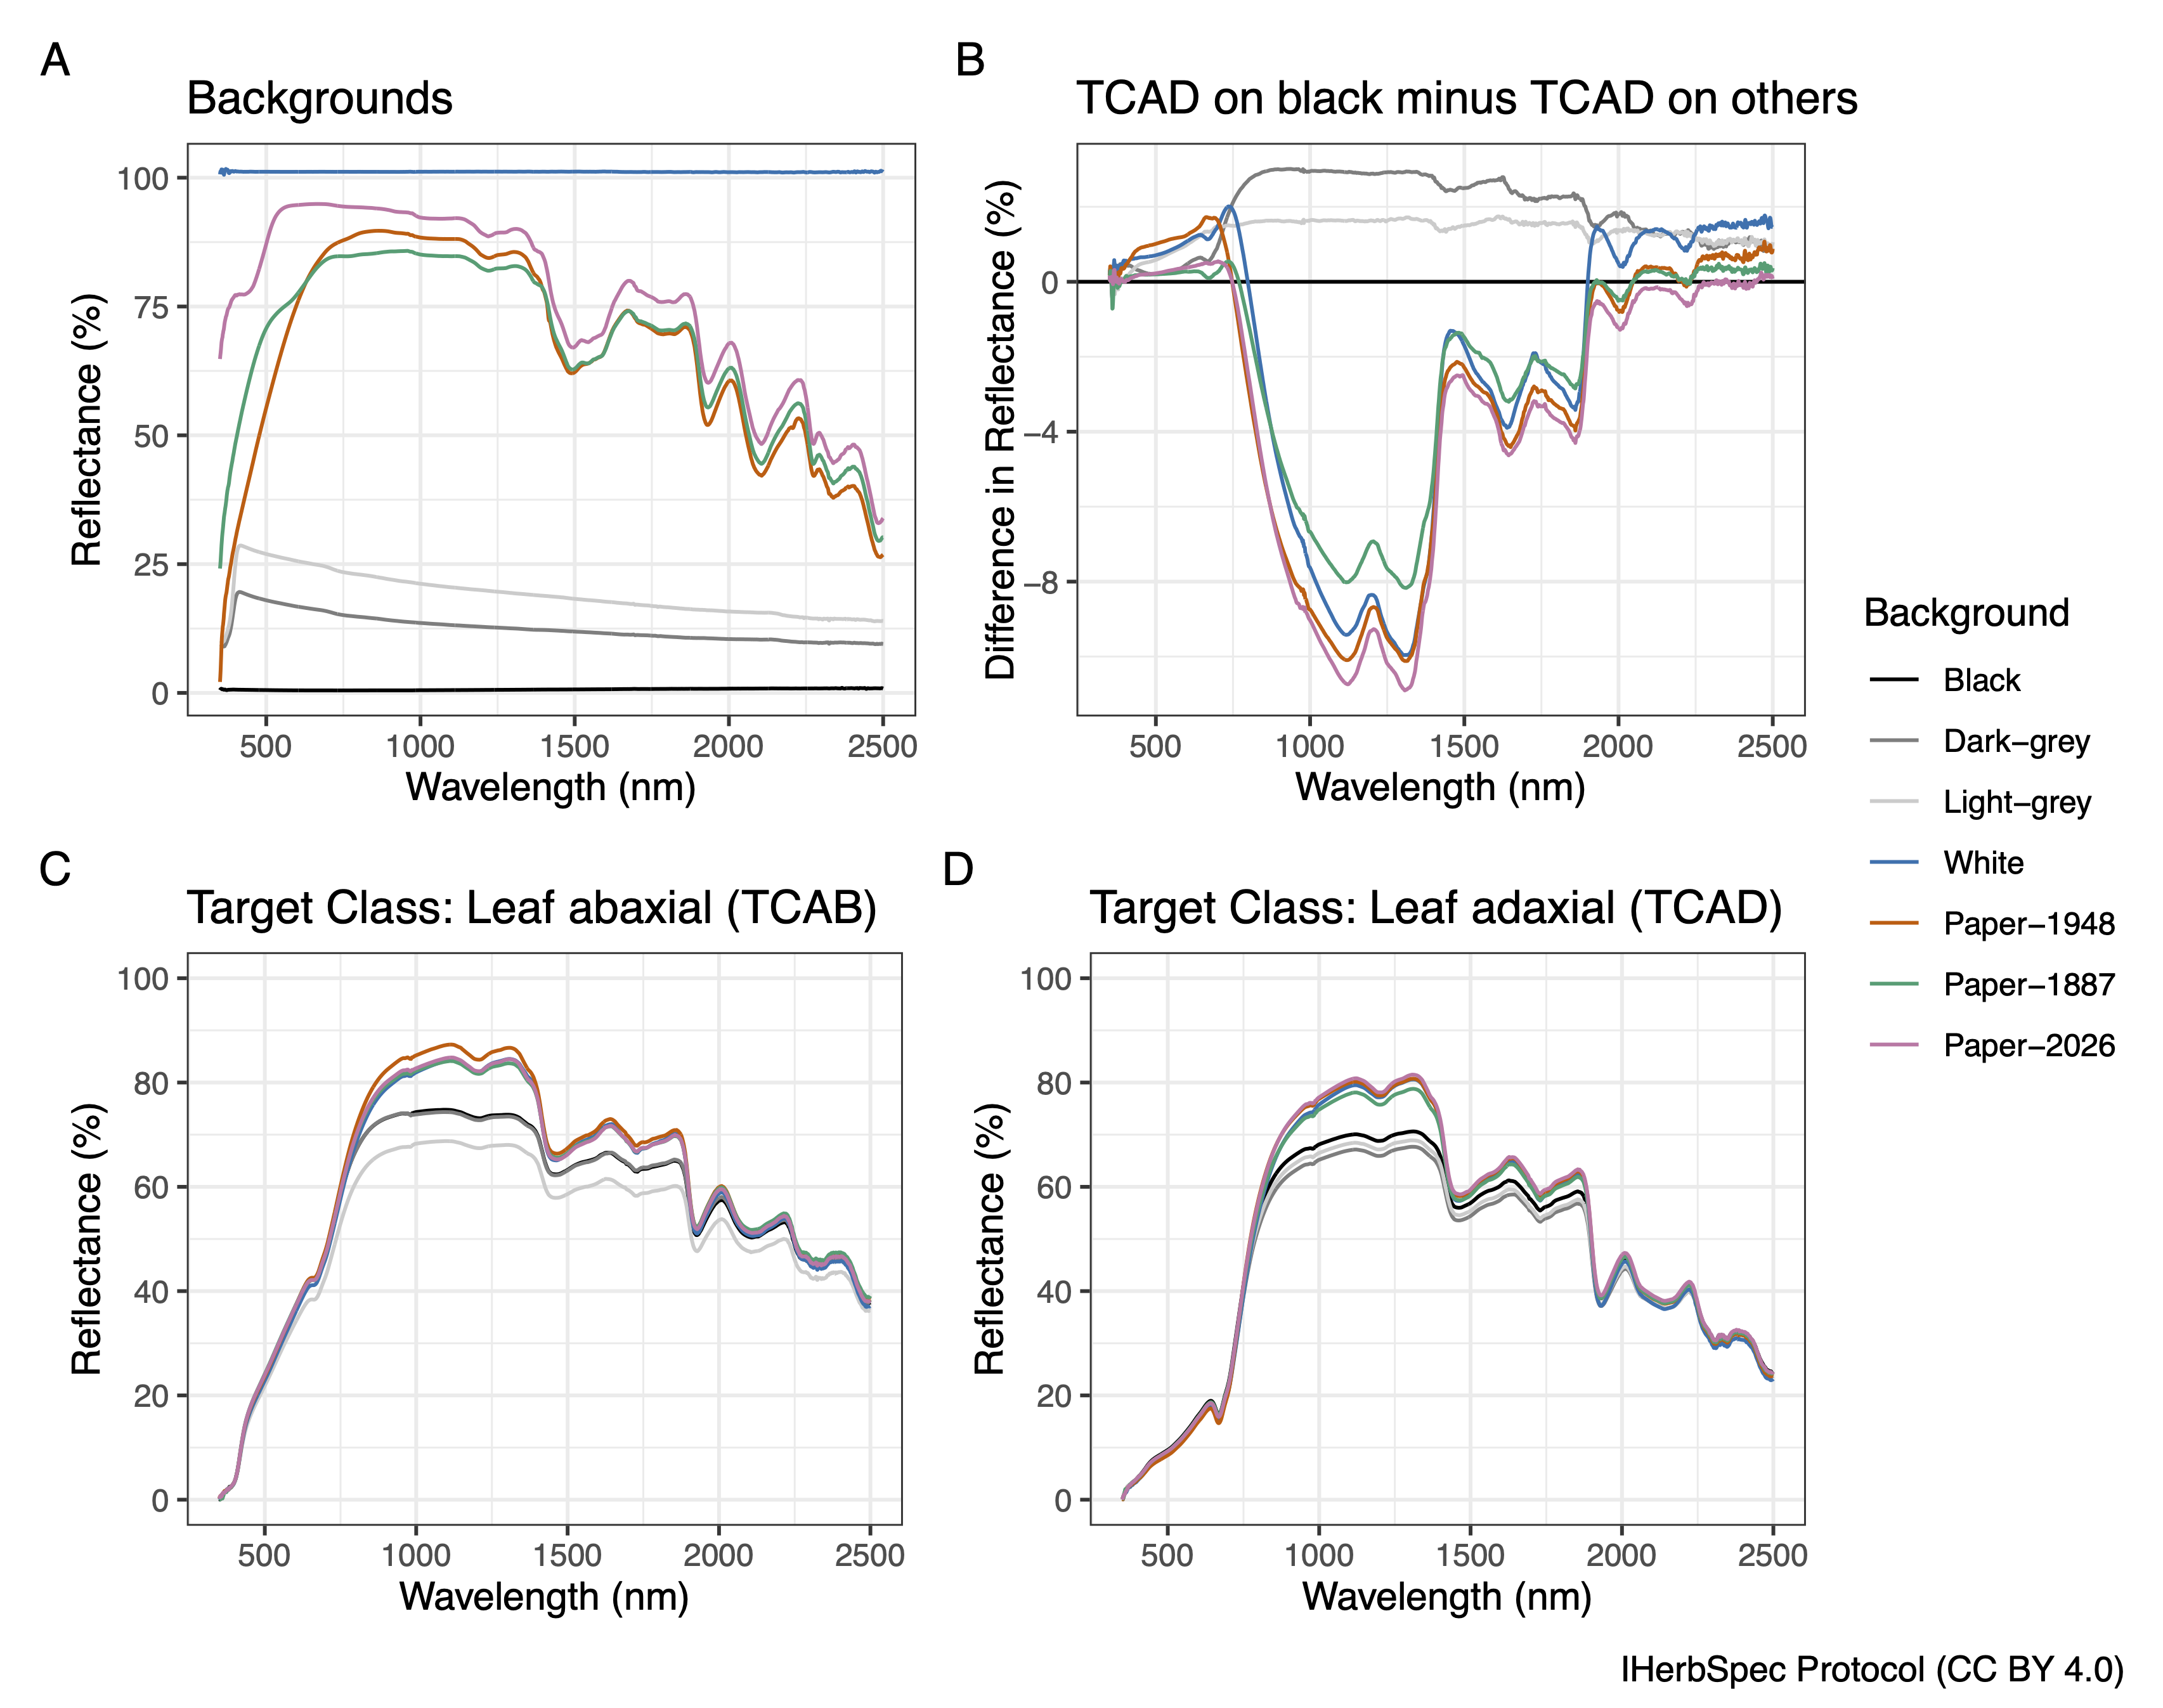
\includegraphics[keepaspectratio]{images/Fig-backgrounds_v2.jpg}}

}

\caption{\textbf{Fig. 5.1.} Reflectance of different background
materials and their effects on target tissue spectra. \textbf{(A)}
Reflectance spectra of common background materials used in herbarium
spectral measurements, including black (Musou IR Flock), dark grey,
light grey (grey matte paint on canvas), white (Spectralon 99\%), and
three herbarium mounting paper types of different ages. Each background
exhibits a distinct spectral profile across the visible--shortwave
infrared range (400---2500 nm). \textbf{(B)} Differences between adaxial
leaf spectra measured on black background (TCAD\_BGB) with spectra of
the same leaf surface measured on the other backgrounds (see legend).
Deviations from zero indicate wavelength-dependent background-induced
biases, which are greatest in the near-infrared (NIR; c.~700---1100 nm)
and shortwave infrared I regions (SWIR 1; 1100---2000 nm). \textbf{(C)}
Reflectance spectra of leaf abaxial surface (TCAB) measured on different
backgrounds, illustrating how background reflectance can influence
absolute reflectance values across spectral regions. \textbf{(D)} Mean
reflectance spectra of leaf adaxial surface (TCAD) measured on different
backgrounds, showing similar background-dependent effects. All
measurements were made with a Spectral Evolution NaturaSpec
spectroradiometer using a handheld herbarium leaf probe.}

\end{figure}%

5.3.3. \textbf{Target measurements of background material (black or
paper) must be linked to tissue measurements using filename conventions
(\hyperref[part-3-filename-conventions-and-formats]{Part 3}).}

\begin{itemize}
\tightlist
\item
  This supports quality control of background conditions and enables
  development of spectral unmixing approaches to isolate tissue
  reflectance.
\end{itemize}

5.3.4. \textbf{Wear gloves and carefully handle all tissues, white
reference, black backgrounds, and calibrated reflectance standards to
keep them clean (see \hyperref[precautions]{5.1 Precautions}).}

5.3.5. \textbf{Calibrated reflectance standards:}

\begin{itemize}
\tightlist
\item
  Institutions should consider purchasing calibrated reflectance
  standards, such as Spectralon® Calibrated (SL Standard) Diffuse
  Reflectance Standards. These should be kept clean and separate from
  `working' white references, and used for long-term assessment of
  instrument performance, optical drift, and the condition of reference
  materials (e.g., white references and black backgrounds).\\
\item
  These are supplied with a calibration certificate and serial number
  that verifies reflectance values across wavelengths.\\
\item
  Reflectance standards are white (e.g., Spectralon® 99\%) and black
  (e.g., Spectralon® 2\%) at a minimum, and can also include gradations
  of gray.\\
\item
  It is recommended that standards be measured at regular intervals
  depending on the level of activity (e.g., once per session; consult
  spectroradiometer manufacturer), and archived with the filename
  conventions provided in \hyperref[tbl-3-1]{Table 3.1}.
\end{itemize}

\section{5.4 Specimen and Tissue
Annotation}\label{specimen-and-tissue-annotation-1}

5.4.1. \textbf{Metadata recommendation:}

\begin{itemize}
\tightlist
\item
  IHerbSpec recommends recording the \texttt{tissueLocation} metadata
  field (see \hyperref[tbl-4-3]{Table 4.3}) to document the position of
  measured tissues on the specimen.
\end{itemize}

5.4.2. \textbf{Consult with herbarium collections managers} to define a
suitable specimen annotation protocol that aligns with institutional
policies.

5.4.3. \textbf{Recommended specimen annotation practices:}

\begin{itemize}
\tightlist
\item
  Attach a project annotation label to the herbarium sheet (e.g., ``Leaf
  spectral reflectance; DM White (2025)'').\\
\item
  Use archival-quality materials for labels and annotations, such as
  acid-free paper.\\
\item
  Use pencil for direct annotation of measured tissues on sheets.\\
\item
  For loose tissues (from packets or envelopes):

  \begin{enumerate}
  \def\labelenumi{\arabic{enumi}.}
  \tightlist
  \item
    Place the measured tissue in a glassine envelope, which is archival
    and thin.\\
  \item
    Include a label inside the envelope indicating the
    \texttt{targetTissueClass} and \texttt{targetTissueId} (see
    \hyperref[tbl-4-3]{Table 4.3}; e.g., ``Tissue TN1'').\\
  \item
    Store the envelope in the specimen packet or attach it to the
    herbarium sheet (see \hyperref[f4-2]{Fig. 4.2}).
  \end{enumerate}
\end{itemize}

\begin{center}\rule{0.5\linewidth}{0.5pt}\end{center}

\section{Navigate the protocol}\label{navigate-the-protocol-5}

\begin{itemize}
\tightlist
\item
  Proceed to \hyperref[part6]{\textbf{Part 6}}
\end{itemize}

Browse additional parts and appendices:

\begin{itemize}
\tightlist
\item
  \hyperref[part1]{\textbf{Part 1}} -- Protocol Overview
\item
  \hyperref[part2]{\textbf{Part 2}} -- Measurement and Metadata Workflow
\item
  \hyperref[part3]{\textbf{Part 3}} -- Filename Conventions and Formats
\item
  \hyperref[part4]{\textbf{Part 4}} -- Metadata and Databasing
\item
  \hyperref[part5]{\textbf{Part 5}} -- Instrumentation and Materials
  Guidelines
\item
  \hyperref[part6]{\textbf{Part 6}} -- Selecting Tissues for Spectral
  Measurement
\item
  \hyperref[references]{\textbf{References}}
\item
  \hyperref[app1]{\textbf{Appendix I}} -- Number of Measurements per
  Tissue
\item
  \hyperref[app2]{\textbf{Appendix II}} -- Tissue Metadata for Quality
  Control
\end{itemize}

\bookmarksetup{startatroot}

\chapter{Part 6 -- Selecting Tissues for Spectral
Measurement}\label{part-6-selecting-tissues-for-spectral-measurement}

\section{6.1 Sources of Variation in Herbarium Plant
Tissues}\label{part6}

Spectral data from herbarium specimens are influenced by two major
sources of variation.

The first is the natural \textbf{biological variation} of phenotypes
constructed through genotype-by-environment interactions that biologists
seek to understand. This includes differences in developmental stage
(e.g., young, mature, senescent), within-individual morphological
variation (e.g., sun vs.~shade leaves), and biotic influences such as
herbivory or pathogens.

The second source is \textbf{herborization-related
variation}---herborization being defined as the process of preserving
plant tissues in an herbarium, from the time of collection through
long-term storage. This includes collection, pressing, drying,
application of preservatives, and subsequent storage conditions. Each of
these steps will affect the spectral data to some extent.

For example, differences in technique (e.g., bagged vs.~immediately
pressed specimens; use of ethanol) and environmental factors during
drying and storage can lead to discoloration, dehydration, tissue
distortion, and contamination from biotic or abiotic agents such as
fungus, glue, or insecticides. Among these, the drying protocol might be
particularly influential: specimens not dried efficiently---especially
in warm, humid conditions---are prone to rot and degradation, which
significantly affects spectral quality. Over time, temperature and
humidity fluctuations may accelerate tissue degradation.

As a result, herbarium specimens exhibit a wide range of tissue
conditions, reflecting both the biology of the living organism and the
varied preservation environments they experience. \textbf{Documenting
these sources of variation as metadata is essential}, as they can be
correlated with model accuracy (Kühn et al.~2024, White et al.~2025) and
can be leveraged to improve the performance of predictive models.

When available, contextual details from specimen labels---such as the
use of ethanol or other treatments---should be captured in metadata. As
it is rare to see such details, botanists should be encouraged to
include preservation protocols on specimen labels.

The metadata fields \texttt{hasGlue}, \texttt{hasNonGlueContamination},
\texttt{measurementFlags}, and \texttt{tissueNotes}
(\hyperref[tbl-4-3]{Table 4.3}), are designed to record the condition of
the tissue within the target measurement area at the time of
measurement. These fields are essential for downstream filtering and
analysis of spectra.

Examples of specimen tissue metadata records are provided in
\href{appendix2.qmd}{Appendix II}.

\section{General Guidelines for Tissue
Selection}\label{general-guidelines-for-tissue-selection}

\emph{Note: Much of this text is tailored to measuring leaf tissues, but
can generally be applied to other tissues.}

\begin{enumerate}
\def\labelenumi{\arabic{enumi}.}
\tightlist
\item
  \textbf{Quality over quantity.}

  \begin{itemize}
  \tightlist
  \item
    Under the goal of broad digitization of herbarium tissues, spectral
    data quality could be considered more important than specimen
    quantity. Targeting higher quality, less degraded specimens will
    yield more informative spectral data.\\
  \item
    If the majority of tissues on a specimen are degraded, damaged, or
    contaminated, that specimen should generally not be measured unless
    it holds particular research value.
  \end{itemize}
\item
  \textbf{Select specimens based on their general tissue condition:}

  \begin{itemize}
  \tightlist
  \item
    For digitization projects focused on broad taxonomic coverage,
    specimens should be evaluated as whole units when determining
    suitability for spectral measurement. Next, technicians should
    prioritize tissues that are both suitable for measurement and
    representative of the overall condition of the specimen, rather than
    selecting isolated tissues that are in unusually good condition.
    This approach helps ensure alignment between the general specimen
    condition and the resulting spectral data, and could avoid biases
    based on assumptions of exceptional tissue conditions. If the
    majority of tissues on a specimen are degraded, damaged, or
    contaminated, that specimen should generally not be measured unless
    it holds particular research value. Conversely, if the specimen
    consists mostly of clean, mature, fully expanded tissues, it is
    appropriate to proceed with measurement---while also considering
    additional measurements, when feasible, to capture variation such as
    developmental stage or damage from herbivory and scoring the
    appropriate metadata for these additional measurements.\\
  \item
    \emph{Caveat:} while the overall condition of the specimen informs
    whether it should be measured, metadata on developmental stage,
    contamination, and tissue condition should always record the
    characteristics of the specific measurement area of the tissue---not
    the specimen as a whole. This ensures metadata accuracy and supports
    high-resolution filtering and analysis. Information about the
    specimen can be recorded in the \texttt{tissueNotes} field
    (\hyperref[tbl-4-3]{Table 4.3}).
  \end{itemize}
\item
  \textbf{Score metadata with care.}

  \begin{itemize}
  \tightlist
  \item
    Metadata collection is a critical component for understanding
    factors affecting spectral data quality and will provide confidence
    during data aggregation.\\
  \item
    Herbaria and research teams should train technicians in specimen
    selection strategies and scoring metadata to reduce subjectivity.
  \end{itemize}
\item
  \textbf{Prioritize:}

  \begin{itemize}
  \tightlist
  \item
    Tissue measurements on black backgrounds.

    \begin{enumerate}
    \def\labelenumii{\arabic{enumii}.}
    \tightlist
    \item
      Detached tissues of appropriate size in fragment packets allow
      full assessment of the presence of glue and access to both leaf
      surfaces.\\
    \item
      For mounted specimens, taped or sewn tissues can have black
      backing inserted beneath (technicians should look for evidence of
      old glue).\\
    \end{enumerate}
  \item
    Specimens with mature tissues (e.g., fully expanded leaves) that are
    clean of biotic or abiotic contaminants.\\
  \item
    Tissues that fill the probe measurement area, even if midvein is
    measured.\\
  \item
    Leaves with flat, complete surfaces and intact laminae.
  \end{itemize}
\item
  \textbf{Avoid:}

  \begin{itemize}
  \tightlist
  \item
    Tissues with glue.\\
  \item
    Tissues attached to herbarium paper such that no black background
    can be inserted beneath the tissue.\\
  \item
    Tissues that are not pressed flat (e.g., deformed, folded, crumpled,
    or abnormal leaves).\\
  \item
    Tissues contaminated by biotic or abiotic agents (e.g., algae,
    lichen, fungus, chemical preservatives, glue).\\
  \item
    Damaged tissues (e.g., by herbivory, pathogens, herborization
    phenomena).\\
  \item
    Midribs and major venation in the leaves, or other types of
    vasculature or intrusions in target tissue.\\
  \item
    If larger tissues are available, avoid smaller tissues that don't
    cover the entire optical probe measurement area.
  \end{itemize}
\item
  \textbf{Measuring small tissues:}\\
  Measuring taxa with naturally small tissues presents unique
  challenges, but several strategies can help obtain representative
  spectral measurements with minimal error.

  \begin{itemize}
  \tightlist
  \item
    Center the probe on multiple areas of the small tissue and collect
    several measurements, then average the values to represent the
    tissue's spectral profile.\\
  \item
    Create a mosaic by arranging multiple small tissue units side by
    side to fill the measurement area. Avoid overlapping tissues, as
    stacking can alter light scattering and distort reflectance values
    (\hyperref[fa1]{Fig. A1}).\\
  \item
    Consider optical setup with small measurement area: For projects in
    the instrument selection phase, Spectral Evolution offers a custom
    optical probe with a 2-mm measurement area compatible with their
    NaturaSpec and PSR spectroradiometers.\\
  \item
    Avoid using narrow angle lenses as these might distort the spectrum
    (\hyperref[fa1]{Fig. A1}).
  \end{itemize}
\item
  \textbf{Multiple individual plants within one herbarium sheet:}

  \begin{itemize}
  \tightlist
  \item
    Each individual plant on a sheet should be demarcated with a unique
    \texttt{specimenId} ( \hyperref[tbl-4-2]{Table 4.2}).
  \end{itemize}
\end{enumerate}

\section{Decision tree for tissue
selection}\label{decision-tree-for-tissue-selection}

\begin{figure}[H]

{\centering \pandocbounded{\includegraphics[keepaspectratio]{images/Fig6.1-decisionTree_v1.png}}

}

\caption{\textbf{Fig. 6.1.} Decision tree diagram for target tissue
selection.}

\end{figure}%

\begin{center}\rule{0.5\linewidth}{0.5pt}\end{center}

\section{Navigate the protocol}\label{navigate-the-protocol-6}

Browse additional parts and appendices:

\begin{itemize}
\tightlist
\item
  \hyperref[part1]{\textbf{Part 1}} -- Protocol Overview
\item
  \hyperref[part2]{\textbf{Part 2}} -- Measurement and Metadata Workflow
\item
  \hyperref[part3]{\textbf{Part 3}} -- Filename Conventions and Formats
\item
  \hyperref[part4]{\textbf{Part 4}} -- Metadata and Databasing
\item
  \hyperref[part5]{\textbf{Part 5}} -- Instrumentation and Materials
  Guidelines
\item
  \hyperref[part6]{\textbf{Part 6}} -- Selecting Tissues for Spectral
  Measurement
\item
  \hyperref[references]{\textbf{References}}
\item
  \hyperref[app1]{\textbf{Appendix I}} -- Number of Measurements per
  Tissue
\item
  \hyperref[app2]{\textbf{Appendix II}} -- Tissue Metadata for Quality
  Control
\end{itemize}

\bookmarksetup{startatroot}

\chapter{References}\label{references}

Cavender-Bares J, White DM, Ahlstrand NI, Austin M, Bastianelli D, Bazan
S, Boughalmi K, Cardinal-McTeague W, Chacón-Madrigal E, Couvreur TLP,
Davis C, Durgante FM, Grace OM, Q JAG, Hansen K, Hernández-Leal MS,
Hopkins MJG, Jackson R, Kothari S, Lee AK, Léveillé-Bourret É,
Pinto-Ledezma J, Casaverde NLQ, Meireles JE, Neto-Bradley B, Nichodemus
CO, Ree RH, Schmull M, Soltis DE, Soltis PS, Tuomisto H, Ustin S,
Vasconcelos CC. 2025. \textbf{Next-generation specimen digitization:
capturing reflectance spectra from the world's herbaria for modeling
plant biology across time, space, and taxa} \emph{New Phytologist}.
\url{https://doi.org/10.1111/nph.70645}.

Durgante FM, Higuchi N, Almeida A, Vicentini A. 2013. \textbf{Species
Spectral Signature: Discriminating closely related plant species in the
Amazon with Near-Infrared Leaf-Spectroscopy}. \emph{Forest Ecology and
Management} 291:240--248.
\url{https://doi.org/10.1016/j.foreco.2012.10.045}.

Hadlich HL, Durgante FM, dos Santos J, Higuchi N, Chambers JQ, Vicentini
A. 2018. \textbf{Recognizing Amazonian tree species in the field using
bark tissues spectra}. \emph{Forest Ecology and Management}
427:296--304. \url{https://doi.org/10.1016/j.foreco.2018.06.002}.

Kühn P, Proß T, Römermann C, Wesche K, Bruelheide H. 2024. \textbf{Using
near-infrared spectroscopy to predict nitrogen and phosphorus
concentrations of herbarium specimens under different storage
conditions}. \emph{Plant Methods} 20:19.
\url{https://doi.org/10.1186/s13007-024-01146-x}.

Mersni J, Bazan S, Baby E, Bonnal V, Bastianelli D. 2025.
\textbf{Protocol for NIR spectra acquisition on herbarium specimen}.
\emph{Agritrop}. \url{https://doi.org/10.18167/agritrop/00880}.

Neto-Bradley BM, Bonnet P, Goëau H, Joly A, Cavender-Bares J, Coomes DA.
2025. \textbf{Using reflectance spectra and Pl@ntNet to identify
herbarium specimens: a case study with \emph{Lithocarpus}}. \emph{New
Phytologist}. \url{https://doi.org/10.1111/nph.70258}.

White DM, Cavender-Bares J, Davis CC, Guzmán Q JA, Kothari S, Robles JM,
Meireles JE. 2025. \textbf{Seeing herbaria in a new light: leaf
reflectance spectroscopy unlocks trait and classification modeling in
plant biodiversity collections}. \emph{New Phytologist}.
\url{https://doi.org/10.1111/nph.70357}.

\begin{center}\rule{0.5\linewidth}{0.5pt}\end{center}

\section{Navigate the protocol}\label{navigate-the-protocol-7}

Browse additional parts and appendices:

\begin{itemize}
\tightlist
\item
  \hyperref[part1]{\textbf{Part 1}} -- Protocol Overview
\item
  \hyperref[part2]{\textbf{Part 2}} -- Measurement and Metadata Workflow
\item
  \hyperref[part3]{\textbf{Part 3}} -- Filename Conventions and Formats
\item
  \hyperref[part4]{\textbf{Part 4}} -- Metadata and Databasing
\item
  \hyperref[part5]{\textbf{Part 5}} -- Instrumentation and Materials
  Guidelines
\item
  \hyperref[part6]{\textbf{Part 6}} -- Selecting Tissues for Spectral
  Measurement
\item
  \hyperref[references]{\textbf{References}}
\item
  \hyperref[app1]{\textbf{Appendix I}} -- Number of Measurements per
  Tissue
\item
  \hyperref[app2]{\textbf{Appendix II}} -- Tissue Metadata for Quality
  Control
\end{itemize}

\bookmarksetup{startatroot}

\chapter{Appendix I -- Considerations Regarding the Number of
Measurements per
Specimen}\label{appendix-i-considerations-regarding-the-number-of-measurements-per-specimen}

\section{Three quality measurements for a mean and variance}\label{app1}

Spectral measurements of plant tissues are highly sensitive to both
instrument configuration and small spatial differences across target
tissue. Changes in the optical probe geometry in relation to the
tissue---such as tilting, poor contact with the leaf surface, partial
coverage of the measurement area (Fig. A1), or micro-contaminants like
debris---can introduce technical errors. In addition, leaf surface
microtopography, anatomical variation, and alterations from
herborization (e.g., drying distortion, discoloration, or degradation)
all contribute to variation in reflectance spectra (Cavender-Bares et
al.~2025).

\begin{figure}[H]

{\centering \pandocbounded{\includegraphics[keepaspectratio]{images/figA1-spectra-errors.jpg}}

}

\caption{\textbf{Fig. A1}: Variability in spectral measurements due to
instrument configuration and technical error. The following spectral
measurements are shown: white calibration standard (red), black
background (orange), standard adaxial measurement with black background
(light green), standard adaxial measurement but with narrow-angle lens
following recalibration (dark green), adaxial measurement where the
tissue did not fully cover the optical field of view (i.e.,
\texttt{backgroundInMeasurement} = \texttt{TRUE}; blue), and a folded
leaf (purple). All measurements were made of the same tissue using an
SVC HR-1024i spectroradiometer.}

\end{figure}%

These considerations support the IHerbSpec Protocol requirement of
collecting a minimum of three representative measurements per adaxial
and abaxial leaf surface, when suitable tissues for both surfaces are
available. Three measurements are necessary to calculate a mean spectrum
and its variance. The protocol further recommends collecting five
measurements per surface to achieve a more robust spectral
characterization and to meet the threshold for improved performance in
classification models. The protocol allows for users to make these
minimum or higher measurements on one leaf, in a single spot or in
several locations, or across many leaves. For other tissue types, at
least three measurements are recommended, with more encouraged when
feasible. Below, we elaborate justification for this recommendation.

\section{Evidence-based justification for minimum and recommended
measurements per
specimen}\label{evidence-based-justification-for-minimum-and-recommended-measurements-per-specimen}

Several studies have demonstrated improved model performance when
multiple measurements per individual specimen are averaged, including
those by Durgante et al.~(2013; Figs. A2, A3), Neto-Bradley et
al.~(2025), and S. Bazan et al.~(Unpubl.). The IHerbSpec Protocol's
recommendation of five measurements is based on empirical evidence that
model accuracy gains tend to stabilize beyond five to ten measurements
per tissue (Fig. A2), although the optimal number may vary depending on
tissue type, instrument sensitivity, and modeling goals. Beyond
classification, IHerbSpec members are investigating how replicate
measurements affect the accuracy and robustness of trait prediction
models, evaluating both the benefits of averaging spectra and the
variation in predicted trait values from unaveraged measurements of the
same tissue.

\begin{figure}[H]

{\centering \pandocbounded{
\includegraphics[keepaspectratio]{images/FigA2-Durgante_2013_Fig-spectra.png}}

}

\caption{\textbf{Fig. A2}: Accuracy of taxonomic discrimination as a
function of the number of averaged measurements per specimen. Three
tissue class datasets are analyzed: combined adaxial and abaxial spectra
(circles), abaxial only (squares), and adaxial only (triangles). Each
point represents the average classification accuracy from 50 replicate
linear discriminant analysis models, using randomized subsampling and
test set validation. Error bars indicate 95\% confidence intervals. The
vertical gray line marks the minimum number of spectral measurements (n
= 5), below which accuracy significantly decreases (Tukey test, P ≤
0.05). Data were collected using an FT-NIR spectrometer (1000--2500 nm)
from 10 species in Lecythidaceae, including eight \emph{Eschweilera} and
two \emph{Corythophora} species. Accuracy increases notably between one
and five spectra per specimen, after which performance stabilizes,
indicating diminishing returns beyond five measurements. This figure is
reproduced from Durgante et al.~(2013) with permission from the
publisher.}

\end{figure}%

\begin{figure}[H]

{\centering \pandocbounded{
\includegraphics[keepaspectratio]{images/FigA3-RMSvsNscans.png}}

}

\caption{\textbf{Fig. A3}: Spectral variability as a function of the
number of measurements averaged per subset. Here, a total of 100
spectral measurements were collected from a single Annona sp. leaf using
an ASD LabSpec Pro spectrometer with handheld probe over a black
background. For each subset size (n = 2--40), repeated random subsets of
n spectra were drawn from the full dataset and averaged to simulate
alternative measurement strategies. The root mean square (RMS) distance
among replicate subset-averaged spectra was then calculated. RMS values
decline sharply as the number of measurements averaged increases,
indicating improved stability of the estimated mean spectrum. Averaging
fewer than five measurements resulted in substantially higher
variability among replicate means, whereas gains diminished beyond
approximately 10--20 measurements. This analysis supported the required
minimum of 10 measurements per specimen for the formal protocol
currently implemented by teams at CIRAD and IRD in France (Mersni et
al.~2025).}

\end{figure}%

Another important recommendation in the IHerbSpec Protocol is to measure
both adaxial and abaxial leaf surfaces. These surfaces differ in anatomy
and function due to evolutionary adaptations for light capture, gas
exchange, and environmental stress. Such structural differences are
consistently reflected in their spectral signatures (see
\hyperref[part-1-overview]{Fig. 1.1}), and we recommend measuring both
surfaces---when suitable tissue is accessible---to capture this
biologically meaningful variation.

Within the context of a large-scale macroevolutionary project focusing
on Annonaceae (ERC GLOBAL project; PI Thomas Couvreur), researchers
aimed to measure spectra on one specimen per species with the intent to
capture as much variation as possible for each specimen. In accordance
with the protocol established at the Centre de Coopération
Internationale en Recherche Agronomique pour le Développement (CIRAD),
researchers decided to make 20 spectral measurements per specimen to
develop their spectral library for 1700 Annonaceae species preserved in
over 30 different herbaria.

This decision was informed by preliminary experiments demonstrating that
spectral stability improves with larger numbers of measurements (Fig.
A3). The choice of 20 spectra was also appropriate because of variation
in the number and size of leaves, allowing for multiple measurements of
multiple leaves or single large leaves that filled an entire herbarium
sheet. It also allowed for poor-quality spectra to be discarded based on
downstream filtering criteria while still retaining a large number of
measurements per specimen.

Overall, given the sensitivity of spectral data, research projects are
encouraged---when feasible---to collect more than five measurements per
tissue, including across different tissue units within an individual.
This enables further assessment of intra-individual spectral
heterogeneity and its impact on downstream analyses.

The marginal cost of additional measurements is relatively low across
instruments, with a single measurement typically completed within 1 to
10 seconds. Nevertheless, determining the appropriate number of
measurements remains a critical design consideration, particularly in
large-scale digitization projects involving significant resource
investment.

\begin{center}\rule{0.5\linewidth}{0.5pt}\end{center}

\section{Navigate the protocol}\label{navigate-the-protocol-8}

Browse additional parts and appendices:

\begin{itemize}
\tightlist
\item
  \hyperref[part1]{\textbf{Part 1}} -- Protocol Overview
\item
  \hyperref[part2]{\textbf{Part 2}} -- Measurement and Metadata Workflow
\item
  \hyperref[part3]{\textbf{Part 3}} -- Filename Conventions and Formats
\item
  \hyperref[part4]{\textbf{Part 4}} -- Metadata and Databasing
\item
  \hyperref[part5]{\textbf{Part 5}} -- Instrumentation and Materials
  Guidelines
\item
  \hyperref[part6]{\textbf{Part 6}} -- Selecting Tissues for Spectral
  Measurement
\item
  \hyperref[references]{\textbf{References}}
\item
  \hyperref[app1]{\textbf{Appendix I}} -- Number of Measurements per
  Tissue
\item
  \hyperref[app2]{\textbf{Appendix II}} -- Tissue Metadata for Quality
  Control
\end{itemize}

\bookmarksetup{startatroot}

\chapter{Appendix II -- Representing Tissue Conditions in Metadata for
Quality
Control}\label{appendix-ii-representing-tissue-conditions-in-metadata-for-quality-control}

This appendix provides a brief discussion and examples of the IHerbSpec
approach for recording metadata pertaining to sources of biological and
herborization variation that affect spectral data.

\section{Scoring metadata for tissue conditions}\label{app2}

As explained in
\hyperref[part-6-selecting-tissues-for-spectral-measurement]{Section
6.1} Sources of Variation, we aim to capture biological variation that
is scientifically meaningful, but the degraded nature of herbarium
specimens requires a careful assessment and annotation of tissue quality
and sources of contamination. The Tissue Metadata fields of,
\texttt{developmentalStage}, \texttt{hasGlue},
\texttt{hasNonGlueContamination}, \texttt{measurementFlags}, and
\texttt{tissueNotes} \hyperref[tbl-4-3]{Table 4.3} are designed to
support quality control of spectral data and enable downstream
filtering.

The codes for enumerating the \texttt{developmentalStage} fields are
provided in \hyperref[tbl-4-4]{Table 4.4}, and the codes for
\texttt{measurementFlags} are described in \hyperref[tbl-4-6]{Table
4.6}.

Technicians should also be aware that some taxa (e.g.~Myrtaceae) or
tropical collections in general may naturally exhibit discoloration or
non-flat, deformed surfaces (e.g., \emph{Gasteranthus atratus}). Such
characteristics do not necessarily indicate tissue degradation and
poor-quality spectral data. In addition, some taxa exhibit more
pronounced discoloration during herborization as a result of their
biology, and such discoloration should not be interpreted as evidence of
poor preservation condition. Some traits also covary; for example, young
leaves wilt and become discolored faster and are more challenging to
press and dry flat, so they may more often be scored as moderately or
poorly preserved.

As a reminder, \textbf{\texttt{measurementFlags} pertain only to the
measurement area}, not the whole tissue unit (e.g., leaf). Since
suitable measurement areas of tissues (see decision tree in
\hyperref[part-6-selecting-tissues-for-spectral-measurement]{Fig. 6.1})
will not contain any contaminants, pathogens, or other damage,
technicians should not be enumerating any codes in the
\texttt{measurementFlags} field. This could differ in projects
collecting measurements pertaining to extended uses of the specimen,
e.g., symbionts, degradation, etc., that might be measuring tissue areas
with these other features.

The specimens and metadata examples in \hyperref[tbl-a-1]{Table A1} have
been selected to guide consistent scoring of these fields during
spectral measurement and promote metadata consistency across projects.
Note that the images do not specify the exact measurement area
corresponding to these metadata fields (as is done in the IHerbSpec
Metadata Spreadsheet for specimen NEBC\_00651639 shown in main text
\hyperref[part-2-measurement-and-metadata-workflow]{Fig. 2.2}).

\subsection{Table A1: Examples for Scoring of Tissue
Conditions.}\label{tbl-a-1}

This table provides example metadata records for herbarium specimens,
illustrating how to score select Tissue Metadata
\hyperref[tbl-4-3]{Table 4.3} related to condition and contamination.
The fields \texttt{developmentalStage}, \texttt{hasGlue},
\texttt{hasNonGlueContamination}, and \texttt{measurementFlags} refer
specifically to the measurement area. Broader observations about the
specimen or other tissues can be recorded in \texttt{tissueNotes} (see
\hyperref[tbl-4-3]{Table 4.3}). Linked specimen images are included,
though they do not indicate the precise measurement area corresponding
to each metadata record.

This table can be downloaded on the
\href{https://iherbspec.github.io/protocol}{iherbspec.github.io/protocol}.

\begin{longtable}[]{@{}
  >{\raggedright\arraybackslash}p{(\linewidth - 10\tabcolsep) * \real{0.2078}}
  >{\raggedright\arraybackslash}p{(\linewidth - 10\tabcolsep) * \real{0.1299}}
  >{\raggedright\arraybackslash}p{(\linewidth - 10\tabcolsep) * \real{0.1299}}
  >{\raggedright\arraybackslash}p{(\linewidth - 10\tabcolsep) * \real{0.1299}}
  >{\raggedright\arraybackslash}p{(\linewidth - 10\tabcolsep) * \real{0.1818}}
  >{\raggedright\arraybackslash}p{(\linewidth - 10\tabcolsep) * \real{0.2208}}@{}}
\toprule\noalign{}
\begin{minipage}[b]{\linewidth}\raggedright
\texttt{herbariumCode\_specimenID}
\end{minipage} & \begin{minipage}[b]{\linewidth}\raggedright
\texttt{developmental} \texttt{Stage}
\end{minipage} & \begin{minipage}[b]{\linewidth}\raggedright
\texttt{hasGlue}
\end{minipage} & \begin{minipage}[b]{\linewidth}\raggedright
\texttt{hasNonGlue} \texttt{Contamination}
\end{minipage} & \begin{minipage}[b]{\linewidth}\raggedright
\texttt{measurement} \texttt{Flags}
\end{minipage} & \begin{minipage}[b]{\linewidth}\raggedright
\texttt{tissueNotes}
\end{minipage} \\
\midrule\noalign{}
\endhead
\bottomrule\noalign{}
\endlastfoot
\href{https://kiki.huh.harvard.edu/databases/specimen_search.php?mode=details&id=794136}{A\_00631088}
& \texttt{mature} & \texttt{TRUE} & \texttt{FALSE} &
\texttt{MediumPreservation} & discolored \\
\href{https://kiki.huh.harvard.edu/databases/specimen_search.php?mode=details&id=834226}{A\_00672503}
& \texttt{mature} & \texttt{FALSE} & \texttt{TRUE} &
\texttt{GoodPreservation} & PathogenPresent \\
\href{https://kiki.huh.harvard.edu/databases/specimen_search.php?mode=details&id=800877}{A\_00746288}
& \texttt{mature} & \texttt{TRUE} & \texttt{FALSE} &
\texttt{MediumPreservation} & Discolored. Glue on loose leaf in
measurement area. \\
\href{https://kiki.huh.harvard.edu/databases/specimen_search.php?mode=details&id=793672}{A\_00772865}
& \texttt{young} & \texttt{FALSE} & \texttt{FALSE} &
\texttt{PoorPreservation} & Measured leaves uneven, mottled, discolored,
breakage \\
\href{https://kiki.huh.harvard.edu/databases/specimen_search.php?mode=details&id=1895126}{A\_2613405}
& \texttt{mature} & \texttt{FALSE} & \texttt{FALSE} &
\texttt{MediumPreservation} & \\
\href{https://kiki.huh.harvard.edu/databases/specimen_search.php?mode=details&id=1915798}{A\_2614928}
& \texttt{mature} & \texttt{uncertain} & \texttt{TRUE} &
\texttt{PoorPreservation} & OrganismPresent \\
\href{https://www.aubot.dk/show_entry.php?CatalogNumber=A.S.Barfod48062&&sp_set=all&identification=Danaea\%20wendlandii}{AAU\_A.S.Barfod48062}
& \texttt{mature} & \texttt{FALSE} & \texttt{TRUE} &
\texttt{MediumPreservation} & MidveinPresent \\
\href{https://www.aubot.dk/show_entry.php?CatalogNumber=I.A.Chacon1199&&sp_set=all&identification=Danaea\%20nodosa}{AAU\_I.A.Chacon1199}
& \texttt{mature} & \texttt{FALSE} & \texttt{TRUE} &
\texttt{MediumPreservation} & AlcoholPresent \\
\href{https://www.aubot.dk/show_entry.php?CatalogNumber=R.C.Moran6023&&sp_set=img&identification=Danaea}{AAU\_R.C.Moran6023}
& \texttt{mature} & \texttt{FALSE} & \texttt{TRUE} &
\texttt{GoodPreservation} & AlcoholPresent \\
\href{https://recolnat.fr/fr/specimens/551558e3-8292-4c78-8af6-1ca695e2d7c1?fromExplore=\%60TRUE\%60}{ALF\_035514}
& \texttt{mature}, \texttt{young} & \texttt{FALSE} & \texttt{FALSE} &
\texttt{GoodPreservation} & \\
\href{https://kiki.huh.harvard.edu/databases/specimen_search.php?mode=details&id=231791}{ECON\_00338371}
& \texttt{young} & \texttt{FALSE} & \texttt{FALSE} &
\texttt{MediumPreservation} & Discolored, wrinkled. Specimen burnt but
not in target area. \\
\href{https://kiki.huh.harvard.edu/databases/specimen_search.php?mode=details&id=395867}{GH\_00611866}
& \texttt{mature} & \texttt{FALSE} & \texttt{FALSE} &
\texttt{MediumPreservation} & Discolored specimen \\
\href{https://drive.google.com/file/d/1Jq1xf6qXY9WzqT3HxjgrvNLRF8hPr3QU/view}{INPA\_142198}
& \texttt{mature} & \texttt{FALSE} & \texttt{FALSE} &
\texttt{MediumPreservation} & discolored, herbivory on specimen \\
\href{https://drive.google.com/file/d/1FNv9fwFMu_FowDtoXSLP4lA5cIDgNI4u/view}{INPA\_179322}
& \texttt{mature} & \texttt{FALSE} & \texttt{FALSE} &
\texttt{GoodPreservation} & \\
\href{https://drive.google.com/file/d/14IQvmZxq2vicLC2M7QoNsNZvEsNO_xse/view}{INPA\_184434}
& \texttt{mature} & \texttt{FALSE} & \texttt{FALSE} &
\texttt{MediumPreservation} & Herbivory on specimen, necrotic leaf \\
\href{https://drive.google.com/file/d/1BE6PCBDtpcImSD5t_suGDkKaDA6fZVWf/view}{INPA\_187932}
& \texttt{mature} & \texttt{FALSE} & \texttt{FALSE} &
\texttt{MediumPreservation} & burnt leaves on specimen \\
\href{https://drive.google.com/file/d/1KoDRZW9sM49NMMON1UMbV33MX3ygsWaE/view}{INPA\_203125}
& \texttt{mature} & \texttt{FALSE} & \texttt{FALSE} &
\texttt{MediumPreservation} & discolored, wrinkled leaves \\
\href{https://drive.google.com/file/d/1S-P4yb8-2nb6taY44eR0sXkO_ImGxr9C/view}{INPA\_218399}
& \texttt{mature} & \texttt{TRUE} & \texttt{FALSE} &
\texttt{PoorPreservation} & discolored, herbivory, wrinkled and burnt
leaves \\
\href{https://drive.google.com/file/d/1xg7fWYeZ_6q-w4WmGzdwfVSiulkIYHtx/view}{INPA\_264413}
& \texttt{mature} & \texttt{FALSE} & \texttt{FALSE} &
\texttt{GoodPreservation} & \\
\href{https://drive.google.com/file/d/1vHpKxEW1N3xl0rEa1RJysfvGJWubZ5Am/view}{INPA\_267597}
& \texttt{mature} & \texttt{FALSE} & \texttt{FALSE} &
\texttt{GoodPreservation} & \\
\href{https://drive.google.com/file/d/1LQQ5cEbOpzctYiUI94GzqUZEu3NJPN6m/view}{INPA\_275373}
& \texttt{mature} & \texttt{FALSE} & \texttt{FALSE} &
\texttt{MediumPreservation} & discolored, mold, grayish spots on older
leaves specimen \\
\href{https://drive.google.com/file/d/1bc4Ye52pVqNwoEuDBFukMT4rVbzuC93n/view}{INPA\_278882}
& \texttt{mature} & \texttt{FALSE} & \texttt{TRUE} &
\texttt{MediumPreservation} & AlcoholPresent \\
\href{https://drive.google.com/file/d/1l5lxkfJ9gvhXsE34NnzWiwpqpif4RCxD/view}{INPA\_4628}
& \texttt{mature} & \texttt{FALSE} & \texttt{TRUE} &
\texttt{PoorPreservation} & PreservativePresent \\
\href{https://drive.google.com/file/d/1V6tDj3iPp0qSokmGIe_tf-g2FJcUll2Z/view}{INPA\_59178}
& \texttt{mature} & \texttt{TRUE} & \texttt{TRUE} &
\texttt{PoorPreservation} & PathogenPresent \\
\href{https://drive.google.com/file/d/1dx2xVCjb6YVd23KBwfPNRK9-R9k7qw2p/view}{INPA\_72939}
& \texttt{mature} & \texttt{TRUE} & \texttt{TRUE} &
\texttt{PoorPreservation} & FungusPresent \\
\href{https://drive.google.com/file/d/1JJeU30mNRJtNqQqWCwi72y5O2A8f9ds2/view}{INPA\_97794}
& \texttt{mature} & \texttt{FALSE} & \texttt{FALSE} &
\texttt{MediumPreservation} & wrinkled leaves \\
\href{https://drive.google.com/file/d/1nF5EyZaAEE1VVB2tsZxCX6QsyQwqdgTJ/view}{INPA264208}
& \texttt{mature} & \texttt{FALSE} & \texttt{FALSE} &
\texttt{MediumPreservation} & Measurement area not flat. Herbivory on
sheet \\
\href{https://recolnat.fr/fr/specimens/a64758d3-7cc2-4032-b54b-280ba3dc91ef?fromExplore=\%60TRUE\%60}{M\_PU681750}
& \texttt{mature} & \texttt{FALSE} & \texttt{uncertain} &
\texttt{MediumPreservation} & Discolored; Alcohol preservation
suspected. \\
\href{https://bellatlas.umn.edu/collections/individual/index.php?occid=3069677&clid=0}{MIN\_332436}
& \texttt{mature} & \texttt{FALSE} & \texttt{FALSE} &
\texttt{MediumPreservation} & MidveinPresent \\
\href{https://bellatlas.umn.edu/collections/individual/index.php?occid=3069026&clid=0}{MIN\_370477}
& \texttt{mature} & \texttt{FALSE} & \texttt{FALSE} &
\texttt{PoorPreservation} & discolored, wrinkled leaves \\
\href{https://bellatlas.umn.edu/collections/individual/index.php?occid=3069134&clid=0}{MIN\_588200}
& \texttt{mature} & \texttt{FALSE} & \texttt{FALSE} &
\texttt{GoodPreservation} & \\
\href{https://kiki.huh.harvard.edu/databases/specimen_search.php?mode=details&id=613103}{NEBC\_00634726}
& \texttt{young} & \texttt{FALSE} & \texttt{FALSE} &
\texttt{PoorPreservation} & Measurement area leaves uneven,
discolored \\
\href{https://kiki.huh.harvard.edu/databases/specimen_search.php?mode=details&id=613000}{NEBC\_00636882}
& \texttt{uncertain} & \texttt{FALSE} & \texttt{TRUE} &
\texttt{PoorPreservation} & PathogenPresent \\
\href{https://kiki.huh.harvard.edu/databases/specimen_search.php?mode=details&id=585980}{NEBC\_00651639}
& \texttt{mature} & \texttt{FALSE} & \texttt{FALSE} &
\texttt{GoodPreservation} & \\
\href{https://kiki.huh.harvard.edu/databases/specimen_search.php?mode=details&id=793836}{NEBC\_00677096}
& \texttt{mature} & \texttt{FALSE} & \texttt{TRUE} &
\texttt{MediumPreservation} & PathogenPresent \\
\href{https://kiki.huh.harvard.edu/databases/specimen_search.php?mode=details&id=800585}{NEBC\_00695035}
& \texttt{mature} & \texttt{FALSE} & \texttt{FALSE} &
\texttt{GoodPreservation} & \\
\href{https://kiki.huh.harvard.edu/databases/specimen_search.php?mode=details&id=800514}{NEBC\_00746092}
& \texttt{mature} & \texttt{FALSE} & \texttt{TRUE} &
\texttt{MediumPreservation} & PathogenPresent \\
\href{https://kiki.huh.harvard.edu/databases/specimen_search.php?mode=details&id=800514}{NEBC\_00898559}
& \texttt{mature} & \texttt{FALSE} & \texttt{FALSE} &
\texttt{GoodPreservation} & \\
\href{https://kiki.huh.harvard.edu/databases/specimen_search.php?mode=details&id=1704329}{NEBC\_02618198}
& \texttt{mature} & \texttt{FALSE} & \texttt{FALSE} &
\texttt{MediumPreservation} & Dark spots on measured leaf \\
\href{https://kiki.huh.harvard.edu/databases/specimen_search.php?mode=details&id=1739124}{NEBC\_02618743}
& \texttt{mature} & \texttt{FALSE} & \texttt{FALSE} &
\texttt{GoodPreservation} & \\
\href{https://sweetgum.nybg.org/science/vh/specimen-details/?irn=355043}{NY\_00042623}
& \texttt{mature} & \texttt{TRUE} & \texttt{FALSE} &
\texttt{GoodPreservation} & \\
\href{https://sweetgum.nybg.org/science/vh/specimen-details/?irn=716096}{NY\_00043385}
& \texttt{mature} & \texttt{FALSE} & \texttt{TRUE} &
\texttt{MediumPreservation} & PathogenPresent \\
\href{https://sweetgum.nybg.org/science/vh/specimen-details/?irn=433163}{NY\_00194824}
& \texttt{mature} & \texttt{FALSE} & \texttt{FALSE} &
\texttt{GoodPreservation} & \\
\href{https://sweetgum.nybg.org/science/vh/specimen-details/?irn=648358}{NY\_00402473}
& \texttt{mature} & \texttt{TRUE} & \texttt{FALSE} &
\texttt{MediumPreservation} & MoldPresent \\
\href{https://sweetgum.nybg.org/science/vh/specimen-details/?irn=602603}{NY\_00709210}
& \texttt{mature} & \texttt{FALSE} & \texttt{TRUE} &
\texttt{MediumPreservation} & PathogenPresent \\
\href{https://sweetgum.nybg.org/science/vh/specimen-details/?irn=1392604}{NY\_01163859}
& \texttt{mature} & \texttt{TRUE} & \texttt{FALSE} &
\texttt{MediumPreservation} & Discolored; herbivory on specimen \\
\href{https://sweetgum.nybg.org/science/vh/specimen-details/?irn=2719809}{NY\_02498899}
& \texttt{mature} & \texttt{TRUE} & \texttt{FALSE} &
\texttt{MediumPreservation} & Discolored~ \\
\href{https://sweetgum.nybg.org/science/vh/specimen-details/?irn=2720050}{NY\_02499746}
& \texttt{mature} & \texttt{FALSE} & \texttt{TRUE} &
\texttt{PoorPreservation} & MoldPresent \\
\href{https://science.mnhn.fr/institution/mnhn/collection/p/item/p00391795}{P\_00391795}
& \texttt{mature} & \texttt{FALSE} & \texttt{uncertain} &
\texttt{MediumPreservation} & wrinkled leaves; possible chemical
preservative. \\
\href{https://recolnat.fr/fr/specimens/963508d0-6708-40ac-a2a2-17854b64a1f8?fromExplore=\%60TRUE\%60}{P\_05198525}
& \texttt{mature} & \texttt{FALSE} & \texttt{TRUE} &
\texttt{PoorPreservation} & FungusPresent \\
\href{https://recolnat.fr/fr/specimens/7a679ebb-c03a-4842-ae7c-d3ed7a932e05?fromExplore=\%60TRUE\%60}{P\_05198660}
& \texttt{mature} & \texttt{FALSE} & \texttt{TRUE} &
\texttt{MediumPreservation} & AlcoholPresent \\
\end{longtable}

\section{Navigate the protocol}\label{navigate-the-protocol-9}

Browse additional parts and appendices:

\begin{itemize}
\tightlist
\item
  \hyperref[part1]{\textbf{Part 1}} -- Protocol Overview
\item
  \hyperref[part2]{\textbf{Part 2}} -- Measurement and Metadata Workflow
\item
  \hyperref[part3]{\textbf{Part 3}} -- Filename Conventions and Formats
\item
  \hyperref[part4]{\textbf{Part 4}} -- Metadata and Databasing
\item
  \hyperref[part5]{\textbf{Part 5}} -- Instrumentation and Materials
  Guidelines
\item
  \hyperref[part6]{\textbf{Part 6}} -- Selecting Tissues for Spectral
  Measurement
\item
  \hyperref[references]{\textbf{References}}
\item
  \hyperref[app1]{\textbf{Appendix I}} -- Number of Measurements per
  Tissue
\item
  \hyperref[app2]{\textbf{Appendix II}} -- Tissue Metadata for Quality
  Control
\end{itemize}




\end{document}
